\documentclass[uplatex, titlepage, dvipdfmx, 12pt, a4paper]{jsreport}
\usepackage{geometry}                		% See geometry.pdf to learn the layout options. There are lots.
\geometry{margin=2.5cm}                   		% ... or a4paper or a5paper or ... 
%\geometry{landscape}                		% Activate for rotated page geometry
\usepackage[parfill]{parskip}    		% Activate to begin paragraphs with an empty line rather than an indent
\usepackage[dvipdfmx]{graphicx}				% Use pdf, png, jpg, or eps§ with pdflatex; use eps in DVI mode		
\usepackage{amssymb}
\usepackage{siunitx}
\setcounter{tocdepth}{3}

\title{ \huge 卒業論文\\ \Huge リングイメージ型検出器(RICH)\\の性能評価}
\author{ \LARGE 戸田 匡哉 \and \LARGE 徳田 恵}
\date{\Large \today}							

\begin{document}
\maketitle
\begin{abstract}
 我々は J-PARCハドロン実験施設の高運動量ビームラインにおいてチャームバリオン分光実験 (J-PARC-E50) を計画している。実験では運動量20 GeV/{\sl c} のビーム粒子と標的との反応で生成する 2$\sim$16 GeV/{\sl c}の高運動量散乱粒子の識別を行う必要がある。この広い運動量領域において粒子識別を行うためにリングイメージチェレンコフ検出器を開発している。\\
 粒子識別性能に関わる角度分解能のうち、収差等の内訳を調べるため、テスト機を用いてSPring-8 のLEPSビームラインにおいてテスト実験を行った。光センサーとしてMPPCアレイを使用し、同時にMPPCの暗電流による角度分解能への影響や電圧依存性を調査した。MPPCアレイは8$\times$8の64セグメントで、各セグメントの大きさが3mm$\times$3mmのものを用いた。実験では空気を輻射体とし、0.95 GeV/{\sl c}の電子・陽電子からのチェレンコフ光を球面鏡によってMPPCアレイ上に結像させた。また、MPPCの動作電圧を0.5Vずつ54.0V-57.5Vの間で変化させ、取得したTDCデータからリングイメージを測定した。\\
 得られたリングイメージからリング中心を決定しイベント毎にチェレンコフ角を計算、角度分解能のhit数依存性から角度分解能をセグメントサイズによる位置分解能$\Delta\theta_{seg}$と、収差などによる分解能$\Delta\theta_{other}$に分けた。セグメントサイズによる位置分解能は用いたMPPCの1セグメントの大きさと球面鏡の焦点距離から計算によって求められ、$\Delta\theta_{seg}=2.80$ mradとなる。収差などによる分解能は、角度分解能のhit数依存性のグラフからフィッティングから見積もり、$\Delta\theta_{other}=3.88 \pm 0.02$ mradとなった。ここから焦点面と検出面の位置のずれや、入射粒子の角度分解能、色収差などに細分し、残ったものを暗電流の影響とした。\\
 また各動作電圧でのイベントごとのhit数から、hit数の電圧依存性とシミュレーションによる再現を行なった。


\end{abstract}
\tableofcontents
\chapter{序論}
\section{チャームバリオン分光実験(E50実験)}
 現在、J-PARCではダイクォーク相関の解明を目的としたチャームバリオン分光実験、E50実験が計画されている。この実験ではビーム運動量20 GeV/{\sl c}の$\pi^-$を液体水素標的に当て、次のチャームバリオン$Y^{*-}_c$生成反応を起こす。
\begin{equation}
\pi^- + p \to Y^{*-}_c + D^{*-}
\end{equation}
この時に生じる$D^{*-}$の崩壊モード
\begin{equation}
D^{*-} \to \overline{D}^0\pi^- \to K^+\pi^-\pi^-
\end{equation}
ここから生じる$K^+, \pi^-, \pi^-$の運動量から$D^{*-}$を再構成し、Missing Mass法によって$Y^{*-}_c$を測定する。

\begin{figure}[htbp]
  \begin{center} 
    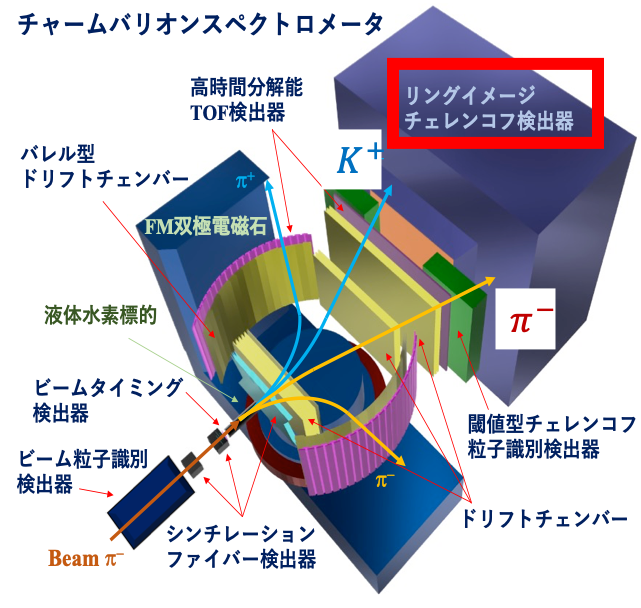
\includegraphics[clip, scale=0.8]{image/E50setup.png}
    \caption{E50実験のセットアップ。図後方のものがリングイメージチェレンコフ(RICH)検出器} 
    \label{fig:E50setup} 
  \end{center}
\end{figure}

$D^{*-}$の一連の崩壊から生じる$K^+, \pi^-$を2$\sim$16 GeV/{\sl c}の広い運動量領域で粒子識別を行う必要がある。そこで用いられるPID検出器が図\ref{fig:E50setup}後方のリングイメージチェレンコフ検出器である。

\section{測定原理}
 荷電粒子が物質中を通過する際にその速度が物質中の光速より早い場合、すなわち次式のような条件を満たす時、円錐状に光が発生する。
\begin{equation}
v > \frac{c}{n} \Leftrightarrow \beta > \frac{1}{n} 
\end{equation}
発生するチェレンコフ光と荷電粒子の進行方向がなす角をチェレンコフ角$\theta_c$と呼び、チェレンコフ角と荷電粒子の速度、物質の屈折率の関係は次式で表される。
\begin{equation}
\cos \theta_c = \frac{1}{n\beta}
\label{cherenkov}
\end{equation}
\begin{figure}[h]
  \begin{center} 
    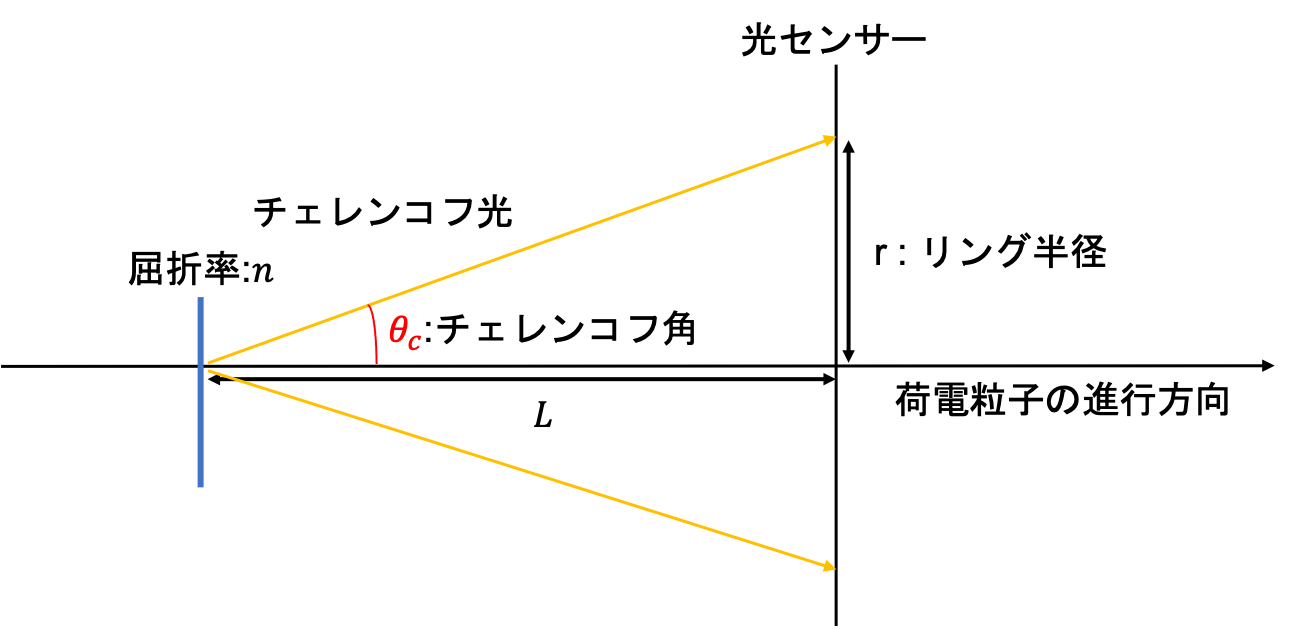
\includegraphics[clip, scale=0.5]{image/cherenkov.png}
    \caption{チェレンコフ光が発生する様子} 
    \label{fig:cherenkov} 
  \end{center}
\end{figure}

リングイメージチェレンコフ検出器では測定したリングイメージの半径と、輻射体から光センサーまでの距離$L$を用いて次の式からチェレンコフ角を算出する。
\begin{equation}
\tan \theta_c = \frac{r}{L} \Leftrightarrow \theta_c = \arctan \left(\frac{r}{L}\right)
\end{equation}
このチェレンコフ角を用いて式(1.4)より、粒子の速度を求めることで粒子識別を行う。
\begin{figure}[htbp]
  \begin{center}
    \begin{tabular}{c}

      % 1
      \begin{minipage}[t]{0.33\hsize}
        \begin{center}
          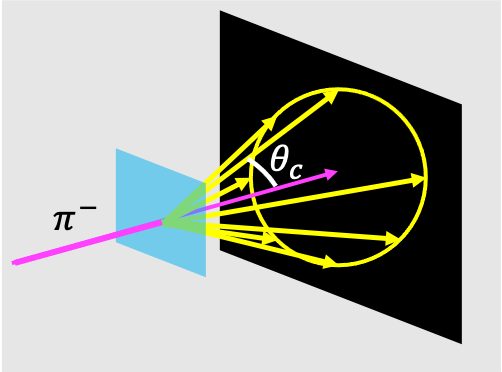
\includegraphics[clip, scale=0.6]{image/pion.png}
          \hspace{1.6cm}
        \end{center}
      \end{minipage}

      % 2
      \begin{minipage}[t]{0.33\hsize}
        \begin{center}
          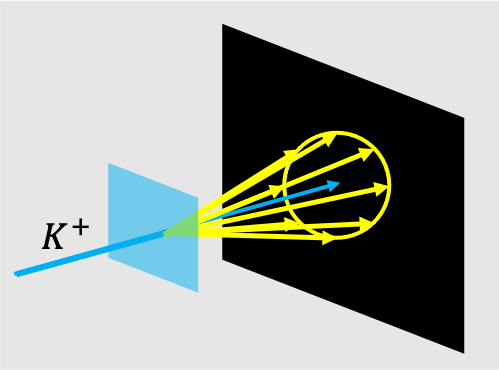
\includegraphics[clip, scale=0.6]{image/kaon.png}
          \hspace{1.6cm}
        \end{center}
      \end{minipage}

    \end{tabular}
    \caption{$\pi^-とK^+によるチェレンコフ光$}
    \label{fig:piKcherenkov}
  \end{center}
\end{figure}

\section{研究目的}
\subsection{先行研究によるRICH検出器実機の構成と要求性能}
 先行研究での実機の構成として、エアロゲル(n=1.04)と$\rm{C_4F_{10}}$ガス(n=1.0037)の2種類の輻射体を用いて、広い運動量領域においてチェレンコフ光を放出させる。このチェレンコフ光を球面鏡で反射させ、光センサー上で収束させることでリングイメージを観測する。

\begin{figure}[htbp]
  \begin{center} 
    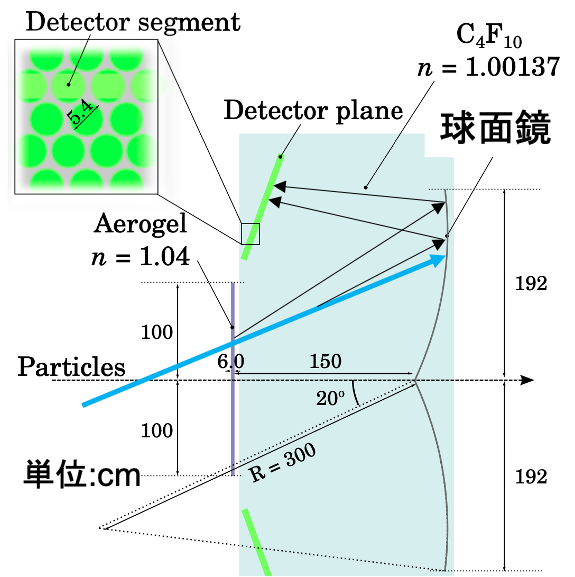
\includegraphics[clip, scale=0.8]{image/RICH.png}
    \caption{実機のデザイン(先行研究より)} 
    \label{fig:RICH} 
  \end{center}
\end{figure}
 実機の要求性能は次のようになっている。目標とする粒子識別性能99\%に要求される角度分解能は$\Delta\theta_c < 10 \rm{mrad}$であり、角度分解能は以下の要素に影響される。
\begin{enumerate}
  \item セグメントサイズの大きさによる位置分解能
  \item 色収差、輻射体の厚さによる分散、検出面での収束等の収差などの影響
  \item ビームの角度分解能
\end{enumerate}
このうち、収差などの影響の内訳は詳細にわかっていないため、球面鏡と光センサーとしてMPPCを用いた小型のテスト機を用いて収差の内訳について調査を行なった。
\subsection{Multi Pixel Photon Counter}
 今回のテスト実験で用いた光センサーであるMulti Pixel Photon Counter、MPPCは安価である、磁場に強いといった利点がある。
一方で熱電子が増幅され、1光電子が常にノイズとして出ており、暗電流が大きいという特徴がある。
その計数率は$100\sim 300\; \si{kHz}$でありRICH検出器では1光電子を捉えるため、その影響についても併せて調査しシミュレーションによる再現を行なった。また電圧によってゲインと検出効率が変わるといった特徴もあり、以降ではMPPCの動作電圧$V_{operation}$から、信号が出始める電圧$V_{breakdown}\sim51V$を引いた$V_{over voltage}$という表記を用いる。
\chapter{実験のセットアップ}
 2020年12月にSPring-8のLEPSビームラインにて実験を行なった。
  実験のセットアップを図(\ref{fig:setup})に示す。
  $\SI{0.95}{GeV/c}$の電子・陽電子をビームとして用い、空気を輻射体とした。
  暗箱内にはビーム軸に対してチェレンコフ光が$15^\circ$の角度で反射するように球面鏡を配置し、MPPC上に焦点を結ぶ様にした。
  暗箱内で発生したチェレンコフ光(青い線)は球面鏡で反射され、MPPCアレイ上に収束される。
  暗箱外側の上流と下流にはトリガーカウンターとして$\SI{10}{mm}$角のプラスチックシンチレーターをそれぞれビーム軸上に配置した。

\begin{figure}[htbp]
  \begin{center} 
    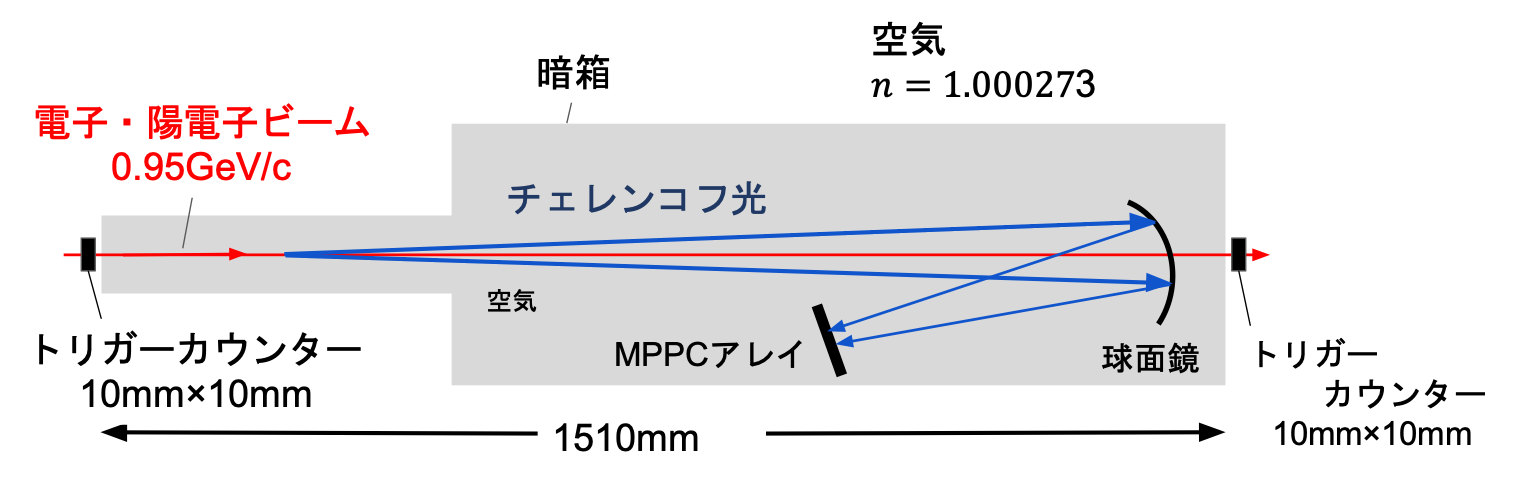
\includegraphics[clip, scale=0.6]{image/setup.png}
    \caption{実験のセットアップ。}
    \label{fig:setup} 
  \end{center}
\end{figure}
MPPCは$8\times8$の2次元アレイ、64セグメントのものを使用し、1セグメントの大きさは$\SI{3.2}{mm}$角である。
動作電圧は$\SI{54}{V}$から$\SI{57.5}{V}$まで$\SI{0.5}{V}$刻みで測定を行なった。読み出しにはNIM-EASIROC moduleを使用し、TDC情報を取得した。
使用した球面鏡は直径が\SI{150}{mm}、曲率半径は\SI{660}{mm}、焦点距離はその半分の\SI{330}{mm}である。

\begin{figure}[htbp]
  \begin{center}
    \begin{tabular}{c}

      % 1
      \begin{minipage}{0.33\hsize}
        \begin{center}
          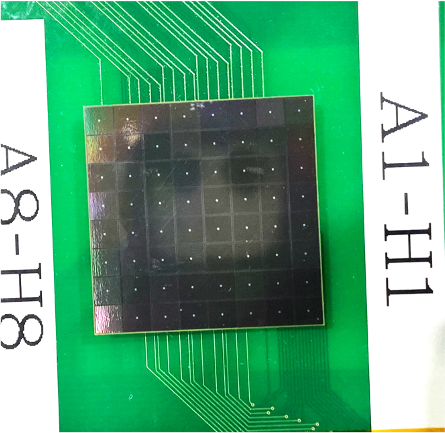
\includegraphics[clip, scale=0.6]{image/MPPC.png}
          \hspace{1.6cm} [1] MPPC
        \end{center}
      \end{minipage}

      % 2
      \begin{minipage}{0.33\hsize}
        \begin{center}
          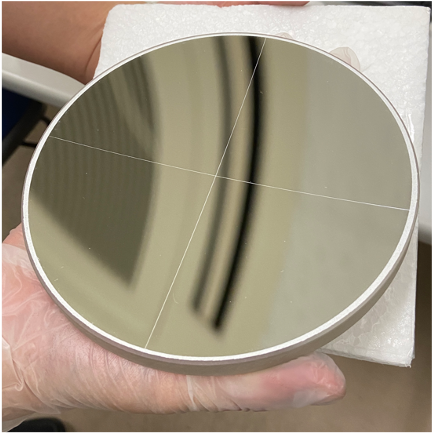
\includegraphics[clip, scale=0.6]{image/mirror.png}
          \hspace{1.6cm} [2] 球面鏡
        \end{center}
      \end{minipage}

    \end{tabular}
    \caption{使用したMPPCと球面鏡。}
    \label{fig:MPPC'N'mirror}
  \end{center}
\end{figure}


\chapter{解析}

\section{hit数}
後述するTDC cutを用いて、1イベント当たりに光子が入ってきたセグメントの数を数え、それをhit数とした。
ただし、今回はTDCでhitの有無のみを見ているため、1セグメントに光子が複数個入っても$\SI{1}{hit}$として数えた。
\begin{figure}[hbtp]
  \begin{center} 
    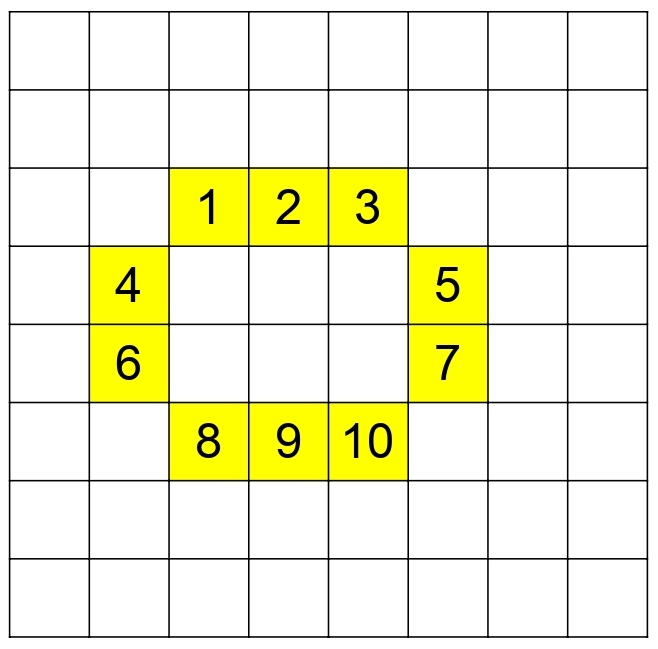
\includegraphics[scale=0.4, clip]{image/hit_image.jpg}
    \caption{あるイベントのhitの様子。光子が入ってきたセグメントを黄色で表している。この場合には$\SI{10}{hit}$と数える。} 
    \label{fig:hit_image} 
  \end{center}
\end{figure}

$V_{ov}=\SI{5}{V}$で各イベントごとにhit数を出し、全イベントのhit数分布のヒストグラムが図\ref{fig:nhits}である。
ヒストグラムのピークをガウスフィットし、そのmeanを各電圧での平均のhit数とした(赤いヒストグラム)。
また、TDCのcutをトリガーのタイミングからズラすことで暗電流によるhit数を見積もった(青いヒストグラム)。
今回は、TDCのcut範囲を$400\sim420\:\si{ch}$にしたときのhit数を暗電流によるhit数とした。

\begin{figure}[hbtp]
  \begin{center} 
    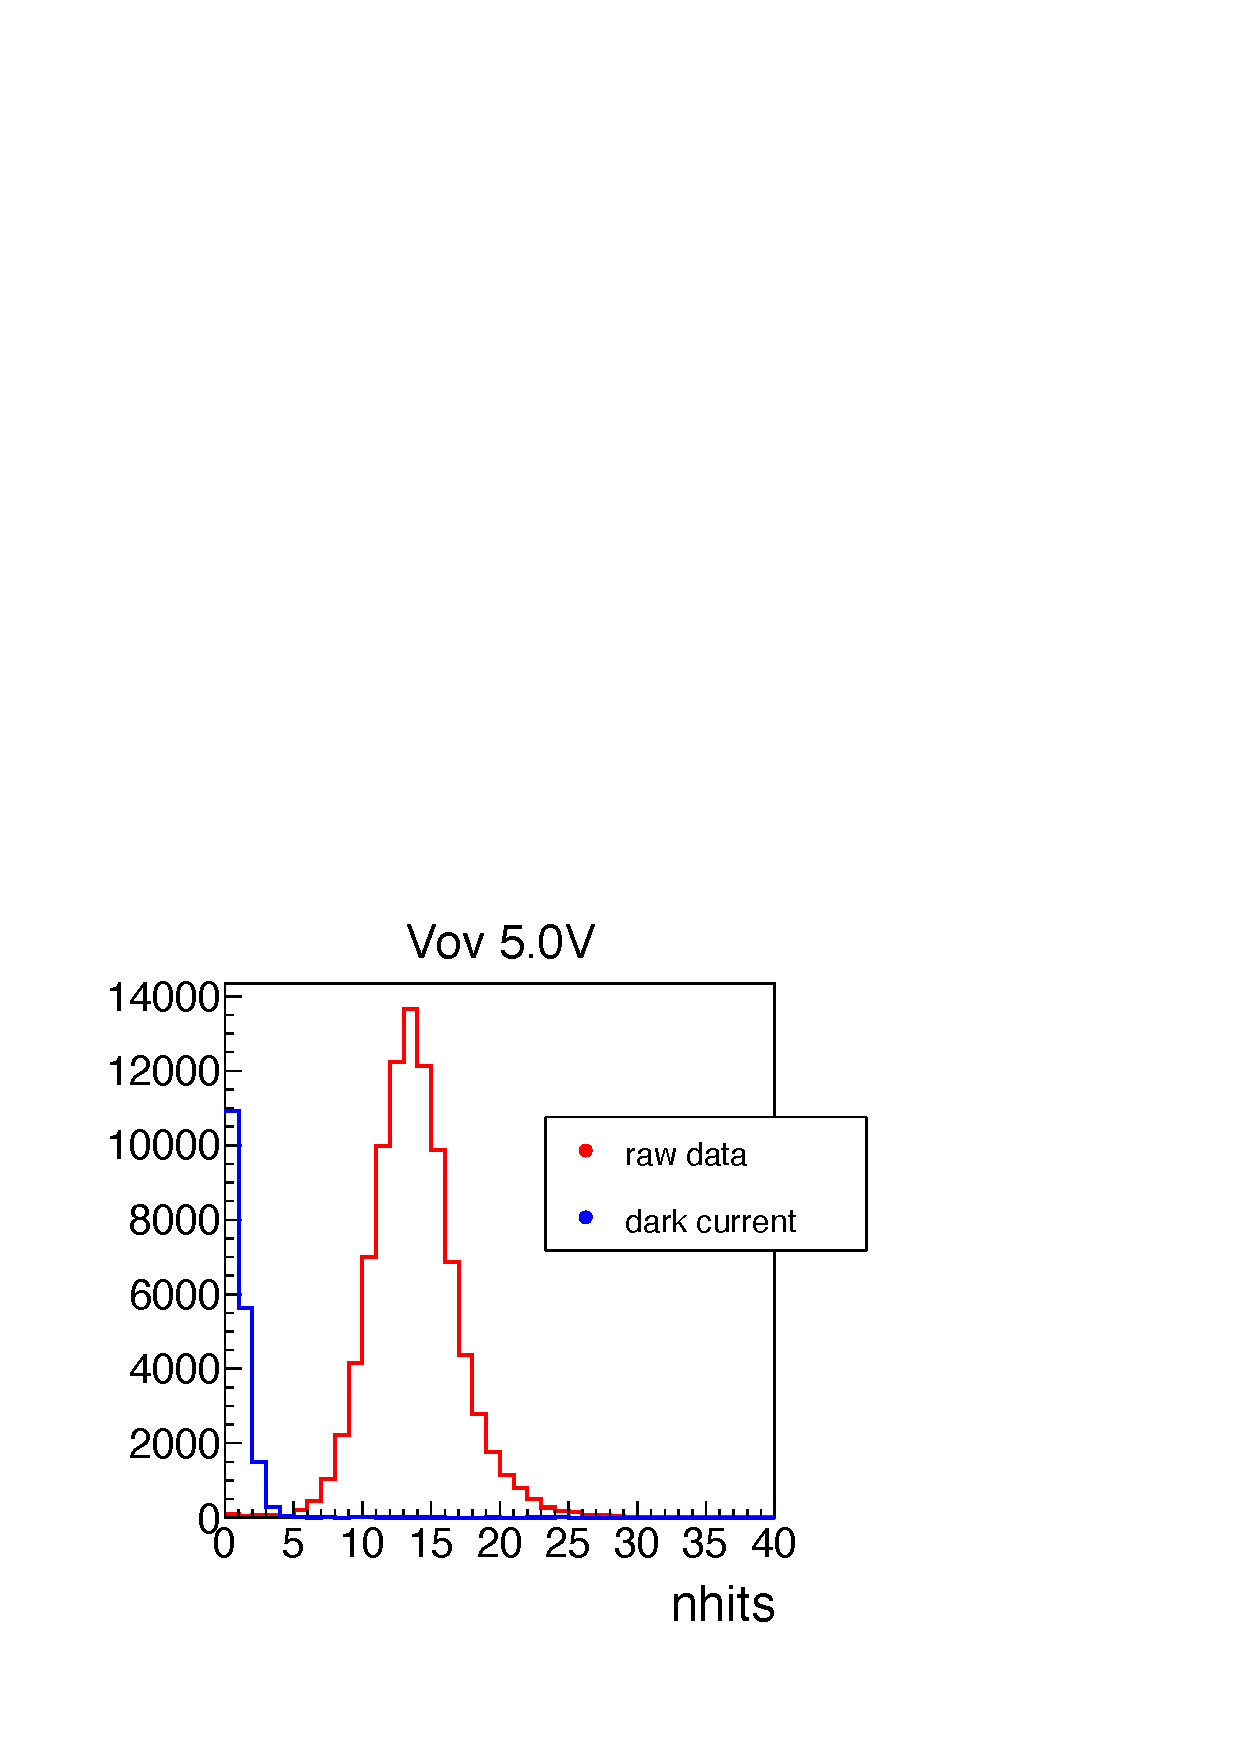
\includegraphics[scale=0.4, clip]{image/Vov5_nhits.pdf}
    \caption{$V_{ov}=\SI{5}{V}$のときのhit数分布} 
    \label{fig:nhits} 
  \end{center}
\end{figure}


  \section{TDC}
   TDCを取得する回路中のディスクリミネーターの閾値は動作電圧が最も低い$V_{ov}=\SI{3.0}{V}$の時の1p.e.に相当する電圧にかけた。
    取得したTDCのヒストグラムが図\ref{fig:tdc}である。
   $\SI{300}{ch}$あたりにピークが確認できる。また、$\SI{290}{ch}$近辺に見られる小さいピークは$\sim\sim\sim$だと考えられる。
  \begin{figure}[htbp]
    \begin{center} 
      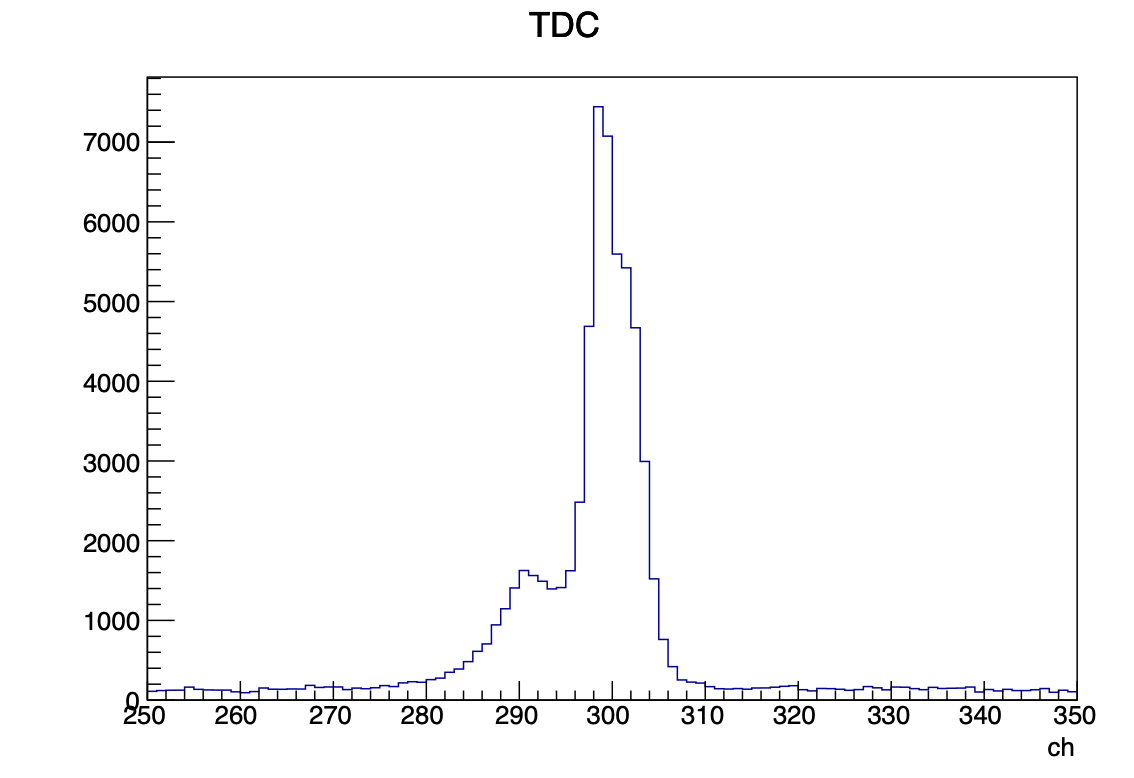
\includegraphics[clip, scale=0.2]{image/tdc.png}
      \caption{得られたTDCのヒストグラム。全てのチャンネルを足し合わせている。}
      \label{fig:tdc} 
    \end{center}
  \end{figure}
  図\ref{fig:tdc}より、今回のTDC cut幅は\SI{21}{ch}と決定した。また、cut positionはcut幅を$\SI{21}{ch}$に固定した状態で
  signal/darkcurrent比が最も良くなるpositionを探して決定した。
  ここで、$signal$は
  \begin{figure}[bthp]
    \begin{center} 
      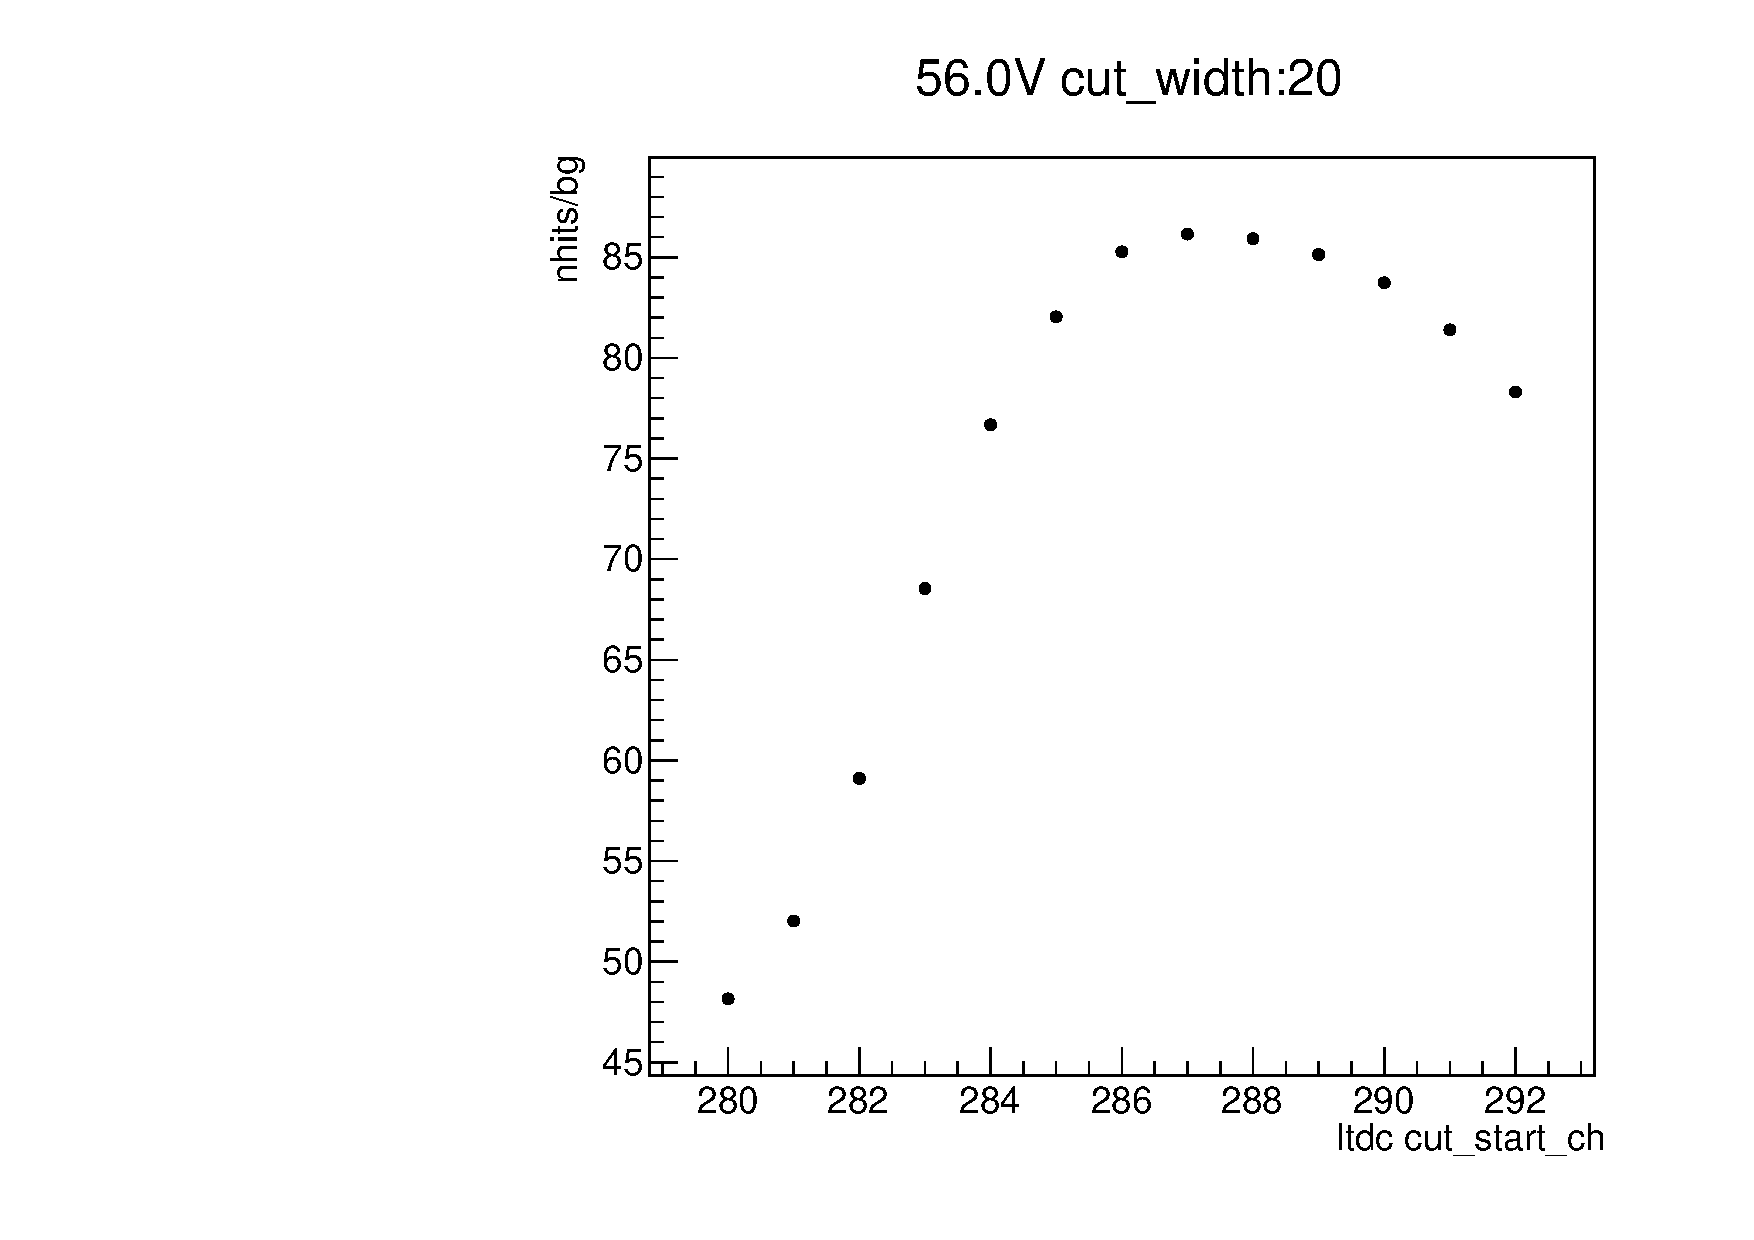
\includegraphics[clip, scale=0.25]{image/TDCcut_scan.pdf}
      \caption{$V_{ov}=\SI{5}{V}$でのscanの様子。横軸はcutのスタート位置でcut幅は$\SI{21}{ch}$で固定している。
      \\ $287\sim 307\;\si{ch}$でsignal/darkcurrent比が最も大きくなっていることが分かる。}
      \label{fig:tdc_scan} 
    \end{center}
  \end{figure}
  図\ref{fig:tdc_scan}より、今回のTDC cut positionは$287 \sim 307 \:\si{ch}$に決定した。
    
  \section{hit patternの確認}
    先ほど求めたhit数をセグメントごとに全イベント分足し上げることで、hit patternを確認したところ、図\ref{fig:hitpattern}のようにチェレンコフリングを確認することができた。
    横軸と縦軸の単位の[array]はMPPCの$8\times 8$セグメントを表している。
    おおよそで中心が(3.5, 4.0)、半径が2だと分かる。(単位はarray)
    \begin{figure}[hbtp]
      \begin{center} 
        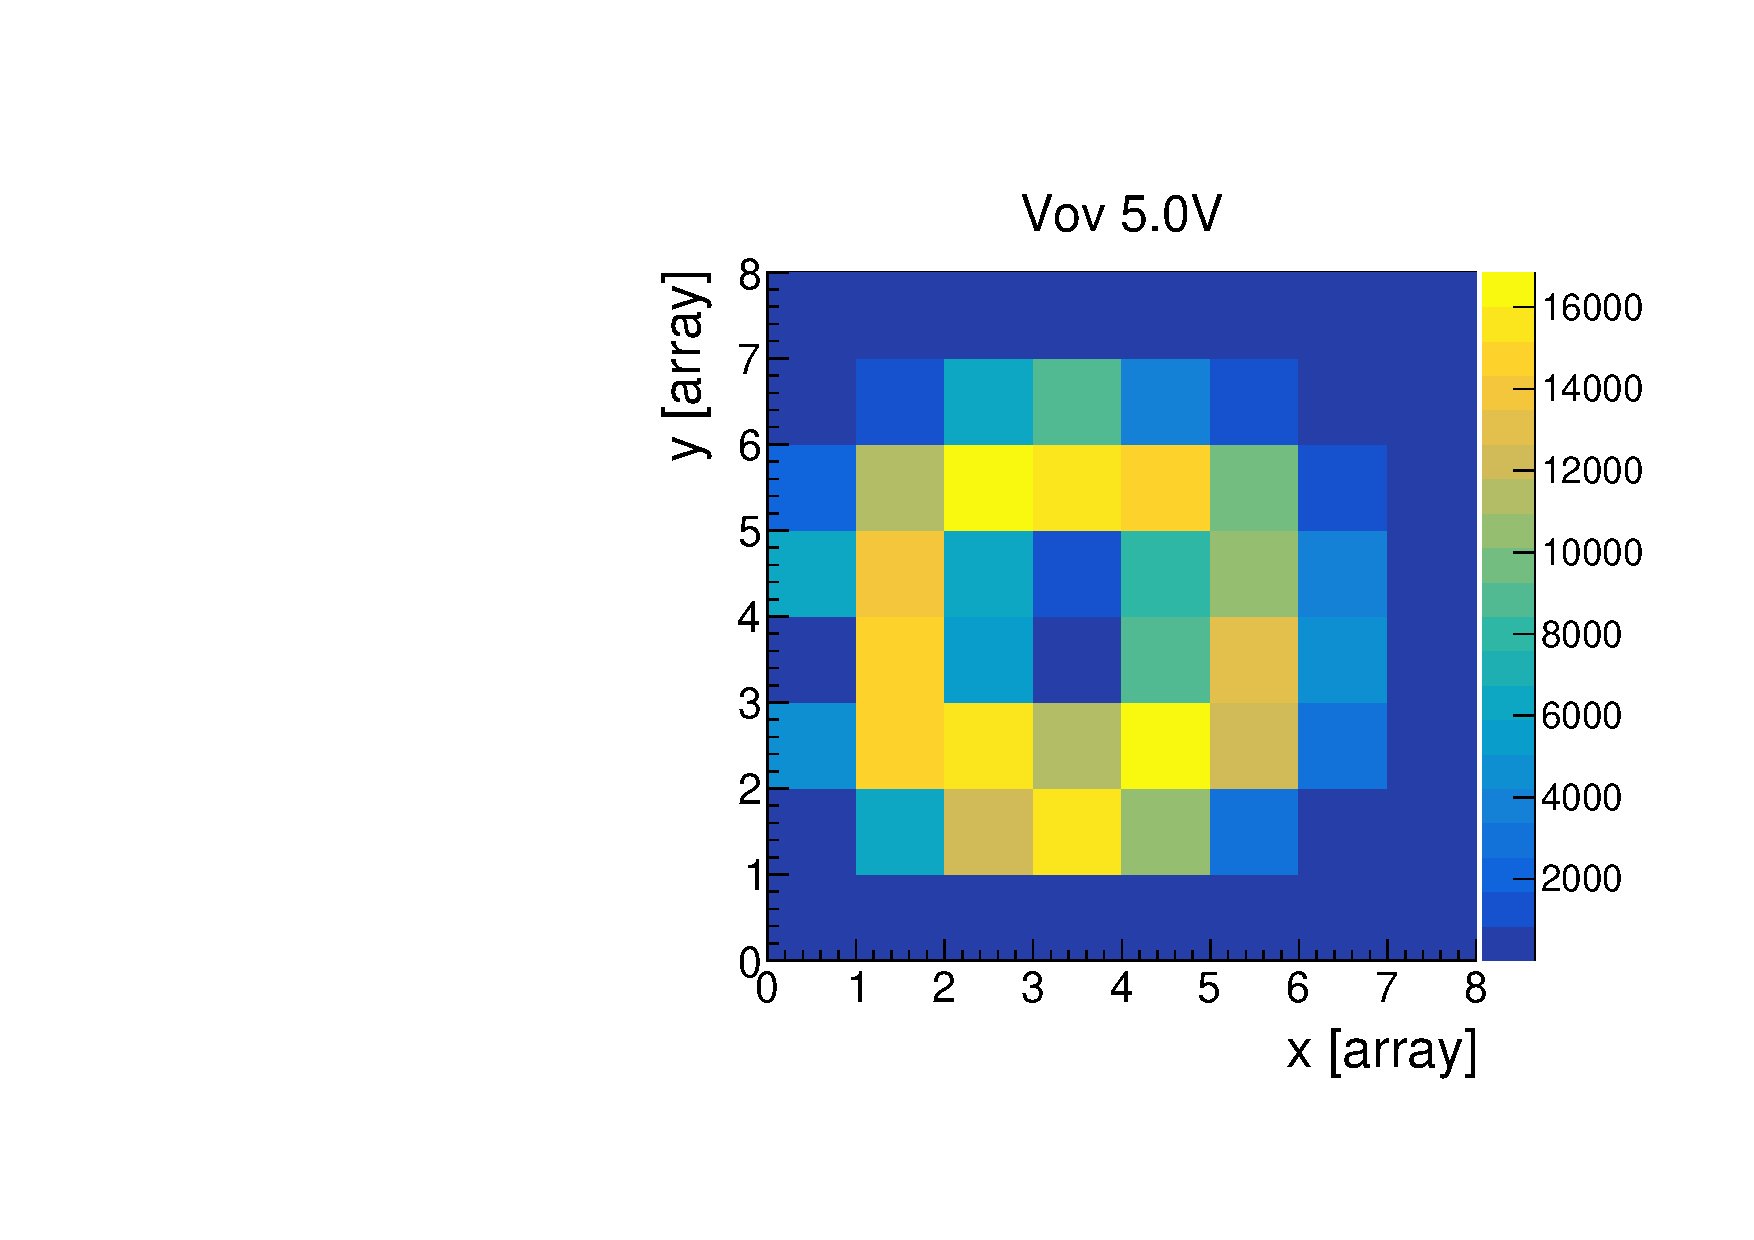
\includegraphics[scale=0.5, clip]{image/hitpattern.pdf}
        \caption{$V_{ov}=\SI{5}{V}$のときのhit pattern} 
        \label{fig:hitpattern} 
      \end{center}
    \end{figure}

  \section{リングイメージの中心}
    図\ref{fig:hitpattern}を見るとわかるように、今回の実験ではアレイの中心とリングの中心がズレていることがわかった。
    実機で使用する際は、リングイメージングチェレンコフ検出器の前方にある飛跡検出器によってリング中心を決定するが、
    今回のテスト機ではリングイメージングチェレンコフ検出器のみなので、セグメントのhitの様子からリング中心を決定する方法を考えた。
    \subsection{リング中心の決定1}
      図\ref{fig:find_center_image}のようにアレイを1列ずつ取り出しセグメントごとのhit数を見ると、円周上に来るセグメントのところで2つのピークが見える。
      また、円周上のyの値がが同じ2点$x_1,x_2$とそのyの値$y_0$の間には円の方程式より、式(\ref{circle_equation})ような関係が成り立つ。
      よって、ピーク間距離$x_2-x_1$を求め、式(\ref{circle_equation})でフィッティングすることで円の中心を求めた。
      ここで、$p_0$はリングの半径、$p_1$はリング中心のy座標を表している。
      
      \begin{equation}
        x_2 - x_1 = 2\sqrt{{p_0}^2-{\left(y_0-p_1\right)}^2}
        \label{circle_equation}
      \end{equation}
      実際のフィッティングの様子が図(\ref{fig:find_ycenter1}),(\ref{fig:find_xcenter1})である。
      黒点が実験データから得られたプロットで、赤線が式(\ref{circle_equation})でフィッティングしたグラフであり、ピークの横軸の値をそれぞれx,yの中心とした。
      この方法では、リングの中心はアレイのマス目を単位として$\left(x,y\right)=\left(3.3, 4.1\right)$と決定された。
      \begin{figure}[hbtp]
        \begin{center}
          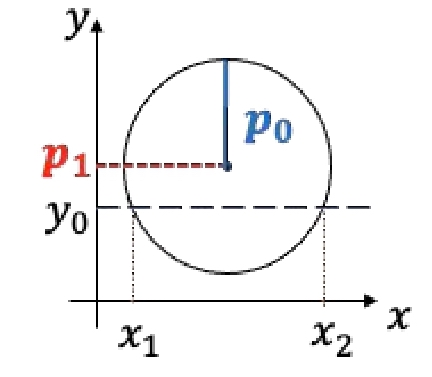
\includegraphics[scale=0.5, clip]{image/find_center1.jpg}
          \caption{yの値を固定した時の図。$x_1, x_2$の2点のピークが見えるので、ピークの間隔から$x_2-x_1$を求める。} 
          \label{fig:find_center_image} 
        \end{center}
      \end{figure}
      \begin{figure}[hbtp]
        \begin{tabular}{cc}
          %---- 最初の図 ---------------------------
          \begin{minipage}[t]{0.45\hsize}
            \centering
            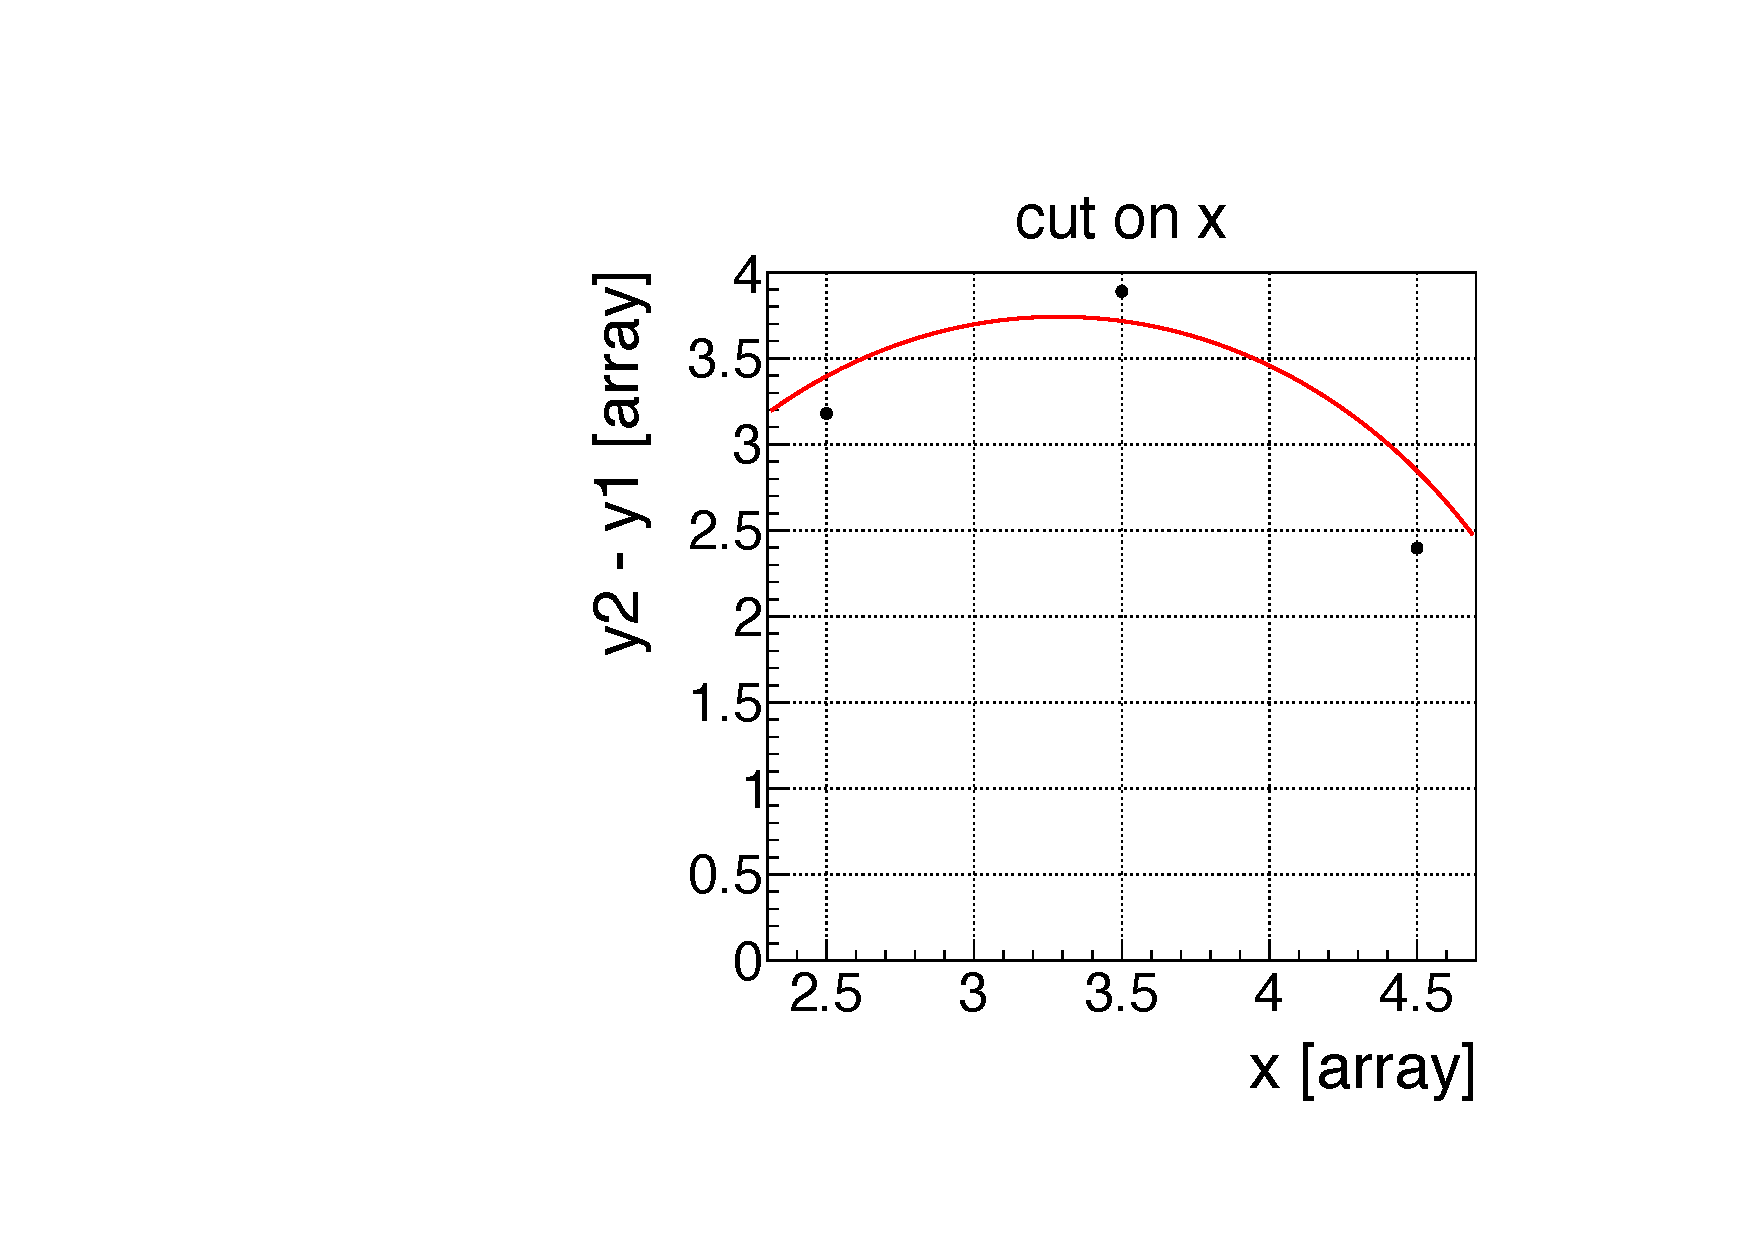
\includegraphics[scale=0.4, clip]{image/find_xcenter.pdf}
            \caption{円を仮定したときの、ある$x$の値に対する$y_2-y_1$の値。} 
            \label{fig:find_xcenter1} 
          \end{minipage}
          %---- 2番目の図 --------------------------
          \begin{minipage}[t]{0.45\hsize}
            \centering
            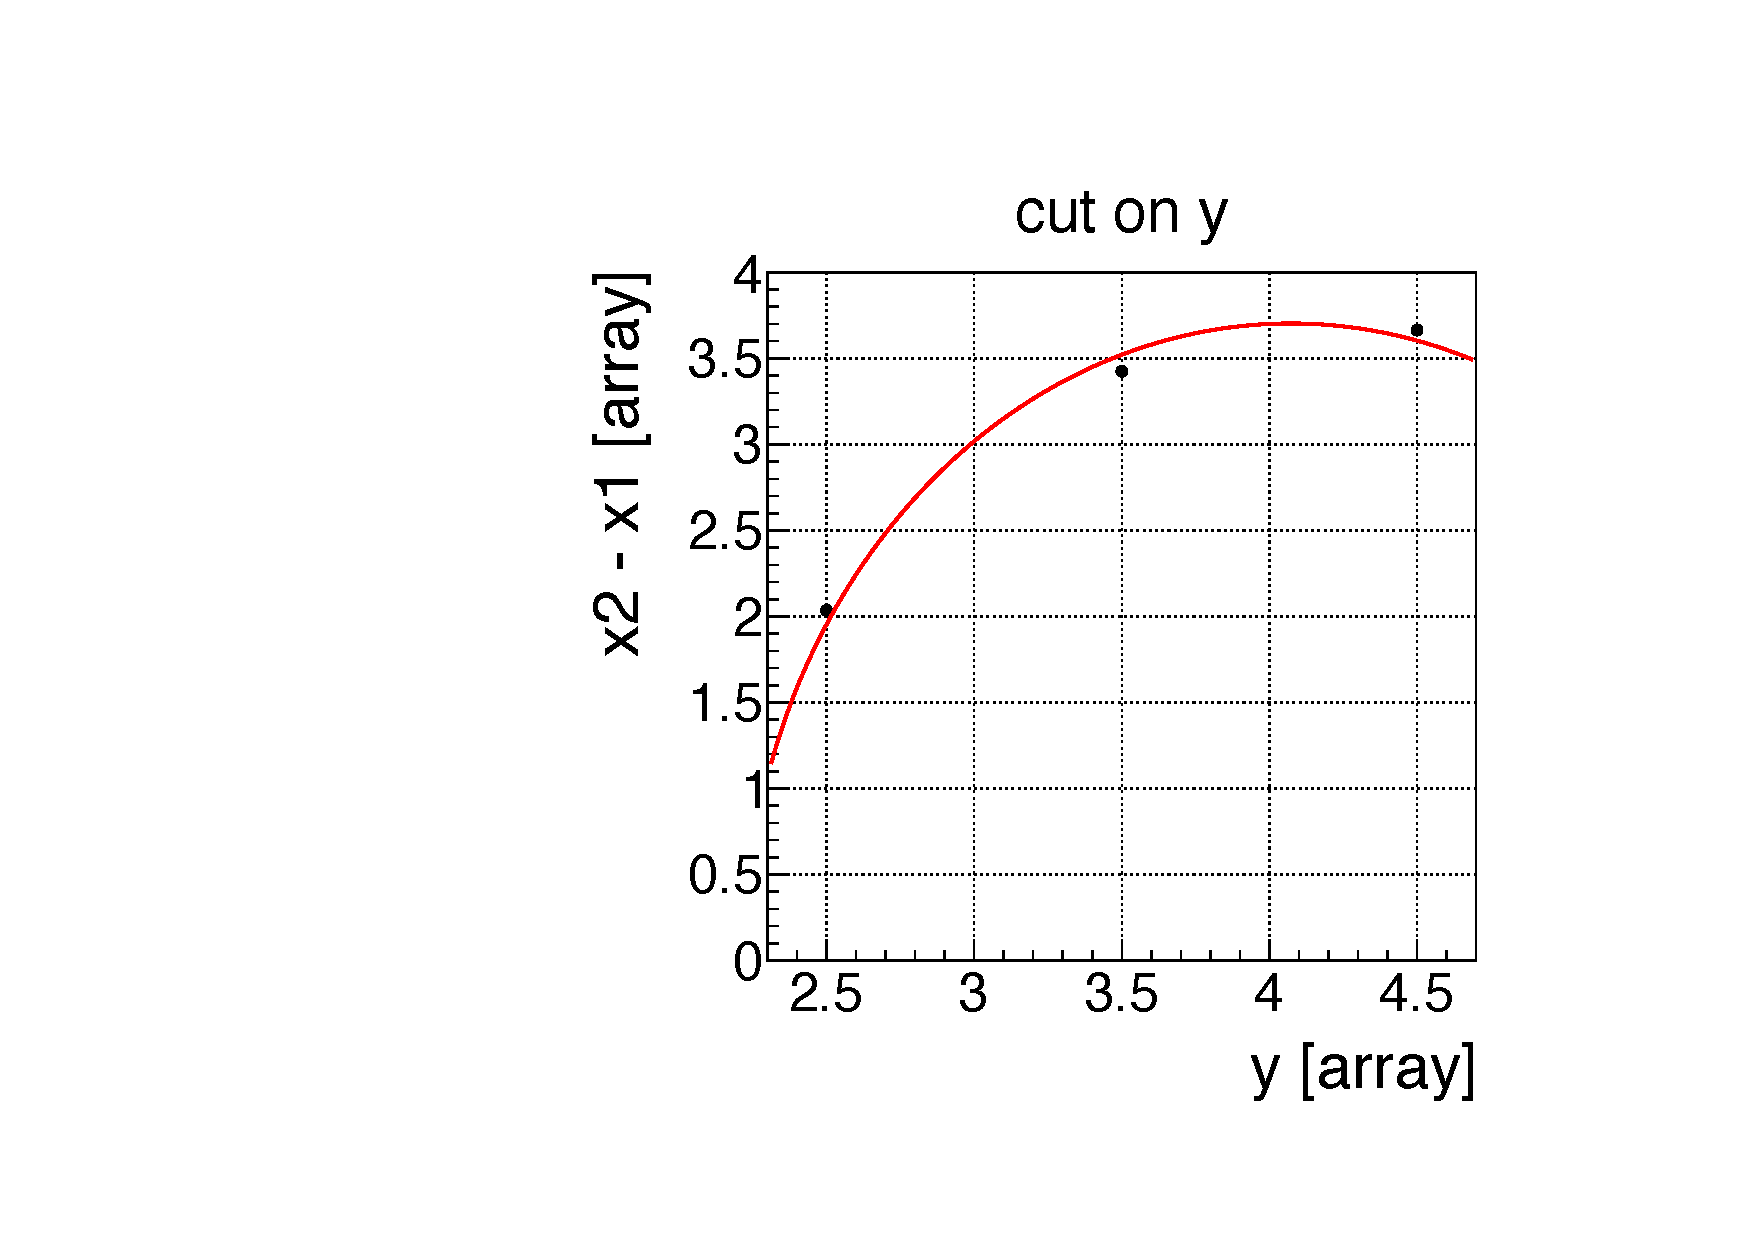
\includegraphics[scale=0.4, clip]{image/find_ycenter.pdf}
            \caption{円を仮定したときの、ある$y$の値に対する$x_2-x_1$の値。} 
            \label{fig:find_ycenter1} 
          \end{minipage} &
          %---- 図はここまで ----------------------
        \end{tabular}
      \end{figure}
    \subsection{リング中心の決定2}
      ここにはリング中心の求め方の二つ目を書く
    \section{リング半径}
    イベントごとに、リング中心からhitしたセグメントまでの距離を平均し、全イベントに対する距離の分布のヒストグラムを描いたのが図(\ref{fig:5Vradius})である。
    1イベントで$n\;\si{hit}$した場合、hitした各セグメントから中心までの距離を$r_1, r_2, \cdots r_n$とすると、そのイベントでの平均半径$r$は
    \begin{equation}
      r = \frac{r_1 + r_2 + \cdots + r_n}{n} \nonumber
    \end{equation}
    となる。
    得られたヒストグラム中のピークをガウスフィットし、meanをその電圧での平均半径とした。
    \begin{figure}[hbtp]
      \begin{center} 
        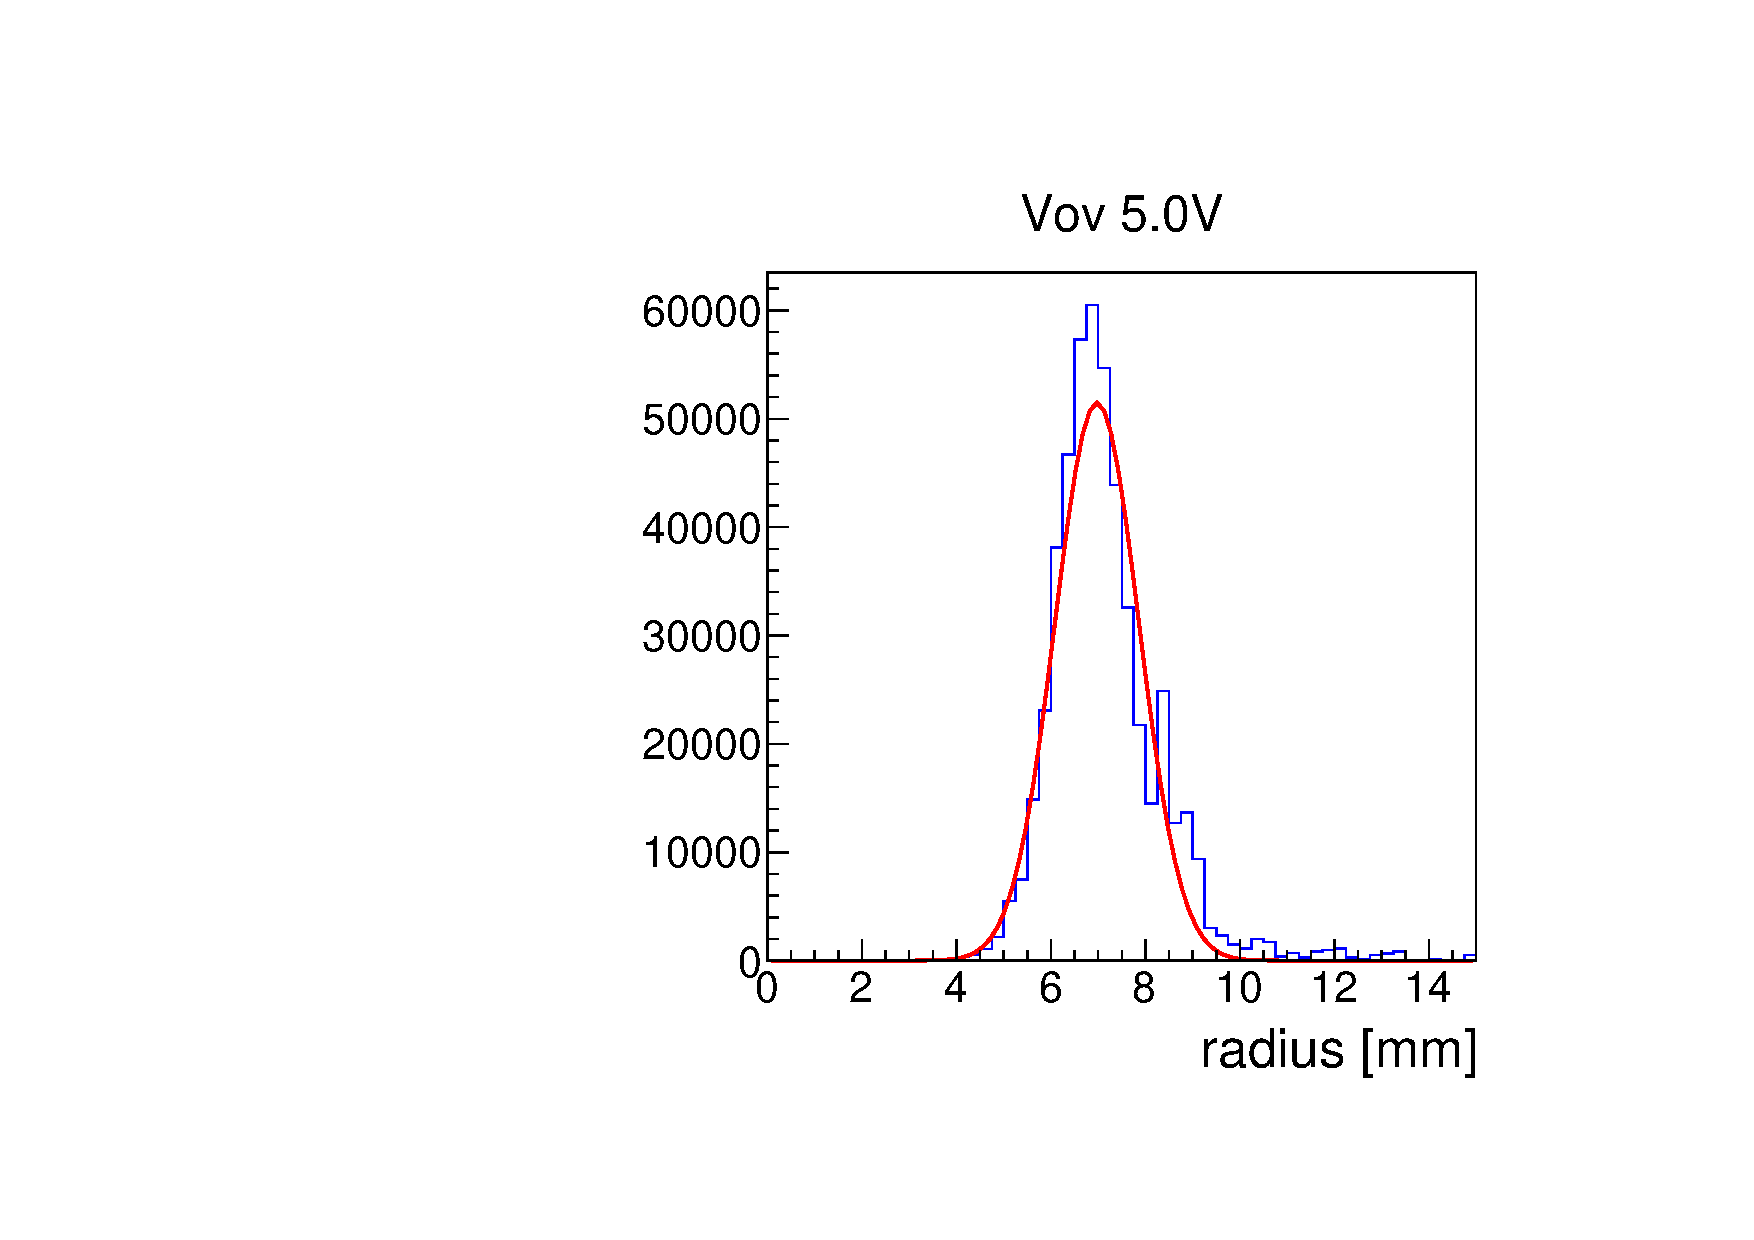
\includegraphics[scale=0.5, clip]{image/radius.pdf}
        \caption{イベントごとに計算したリング半径の分布。} 
        \label{fig:5Vradius} 
      \end{center}
    \end{figure}
    
    
    
    \section{チェレンコフ角と角度分解能}
    チェレンコフ光の式より、チェレンコフ角$\theta_{c}$は、鏡の焦点距離$f$とリング半径$r$を用いて次のように表せる。
    \begin{equation}
      \theta_{c} = \arctan \left(\frac{r}{f} \right)
      \label{theta_radius}
    \end{equation}
    式(\ref{theta_radius})より、イベントごとのリング半径からイベントごとのチェレンコフ角$\theta_{c}$を計算し、全イベントに対するチェレンコフ角$\theta_c$の分布を描いたのが図(\ref{fig:5Vangle})のヒストグラムである。
    そのヒストグラム中のピークをガウスフィットすることでmeanとsigmaを求め、meanをその電圧での平均チェレンコフ角、sigmaをその電圧での角度分解能とした。
    \begin{figure}[hbtp]
      \begin{center} 
        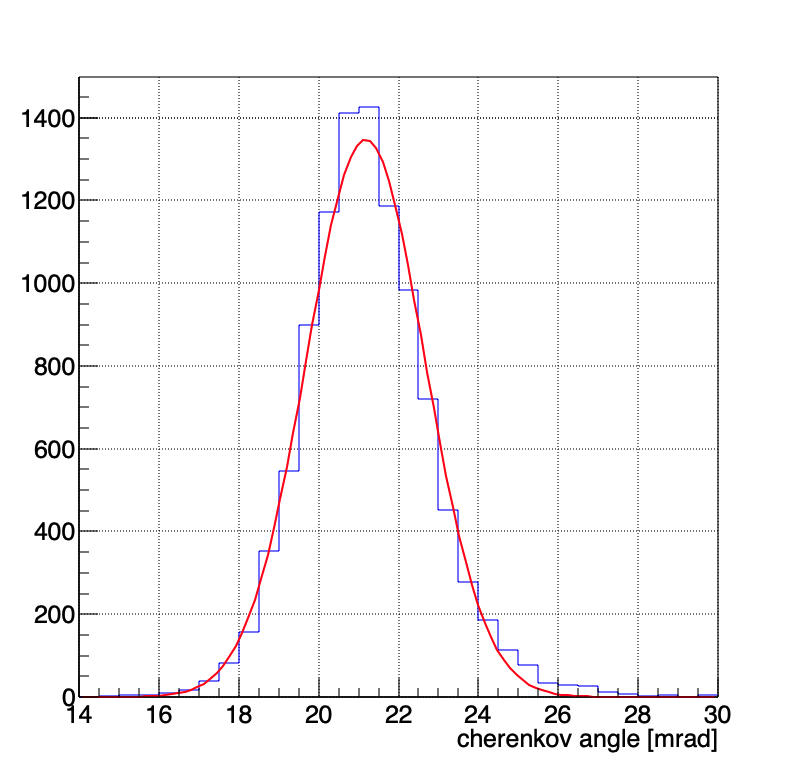
\includegraphics[scale=0.5, clip]{image/Vov5V_angle.png}
        \caption{$V_{ov}=\SI{5}{V}$のときのチェレンコフ角。} 
        \label{fig:5Vangle} 
      \end{center}
    \end{figure}
    
      

\chapter{結果}
  \section{hit数}
    全電圧でのhit数をまとめると、図\ref{fig:hit_dark}の様に$V_{ov}=\SI{5}{V}$付近でサチュレーションしていることがわかる。
    そこで、このサチュレーションしているhit数がもっともらしいかどうかを計算により確かめた。\\
    チェレンコフ光の発生光子数$N_{0}$は、次の式で求めることができる。
    \begin{equation}
        N_{0} = 2 \pi \alpha L  \left(1 - \frac{1}{(n\beta)^2}\right) \frac{1}{\lambda_1\lambda_2} \\
        \label{hit_count1}
    \end{equation}
    ここで、$\alpha$は微細構造定数、$n$は輻射体の屈折率、$\beta$は粒子の速度、$L$は輻射体の長さ、$\lambda_{1}$,$\lambda_{2}$はMPPCの感度のある波長である。
    ただし、実際に検出される光子数$N_{det}$は式(\ref{hit_count2})の様に、この$N_{0}$に鏡の反射効率$\epsilon_{mirror}$やMPPCの量子効率$\epsilon_{MPPC}$を考慮する必要がある。
    \begin{equation}
        N_{det} = \int^{\lambda_2}_{\lambda_1} N_{0}\left(\lambda\right) \epsilon_{mirror}\left(\lambda\right) \epsilon_{MPPC}\left(\lambda\right) d\lambda
        \label{hit_count2}
    \end{equation}
    また、今回は1つのセグメントに同時に複数個の光子が入ってきても$\SI{1}{hit}$と数えるので、いくつかの光子を数え落としてしまう可能性がある。
    式(\ref{hit_count2})より検出光子数を計算し、シミュレーションによって消えてしまう光子数の見積もりも行った。
    具体的には、hit patternからリング上に来ているセグメントを決定し、そのセグメントに計算された検出光子数をランダムに振り分け、セグメントが被ってしまう光子数を消える光子数とした。
    シミュレーションの結果が図\ref{fig:hit_simulation}で、バツ印がシミュレーションで見積もられた光子数、点が実際のデータの値である。
    図(\ref{fig:hit_simulation})より、サチュレーションしているところでは解析値と一致していることがわかった。
    このことから、MPPCの使用は$V_{ov} \ge \SI{5}{V}$が良いことが分かった。
    \begin{figure}[hbtp]
      \begin{tabular}{cc}
        %---- 最初の図 ---------------------------
        \begin{minipage}[t]{0.45\hsize}
          \centering
          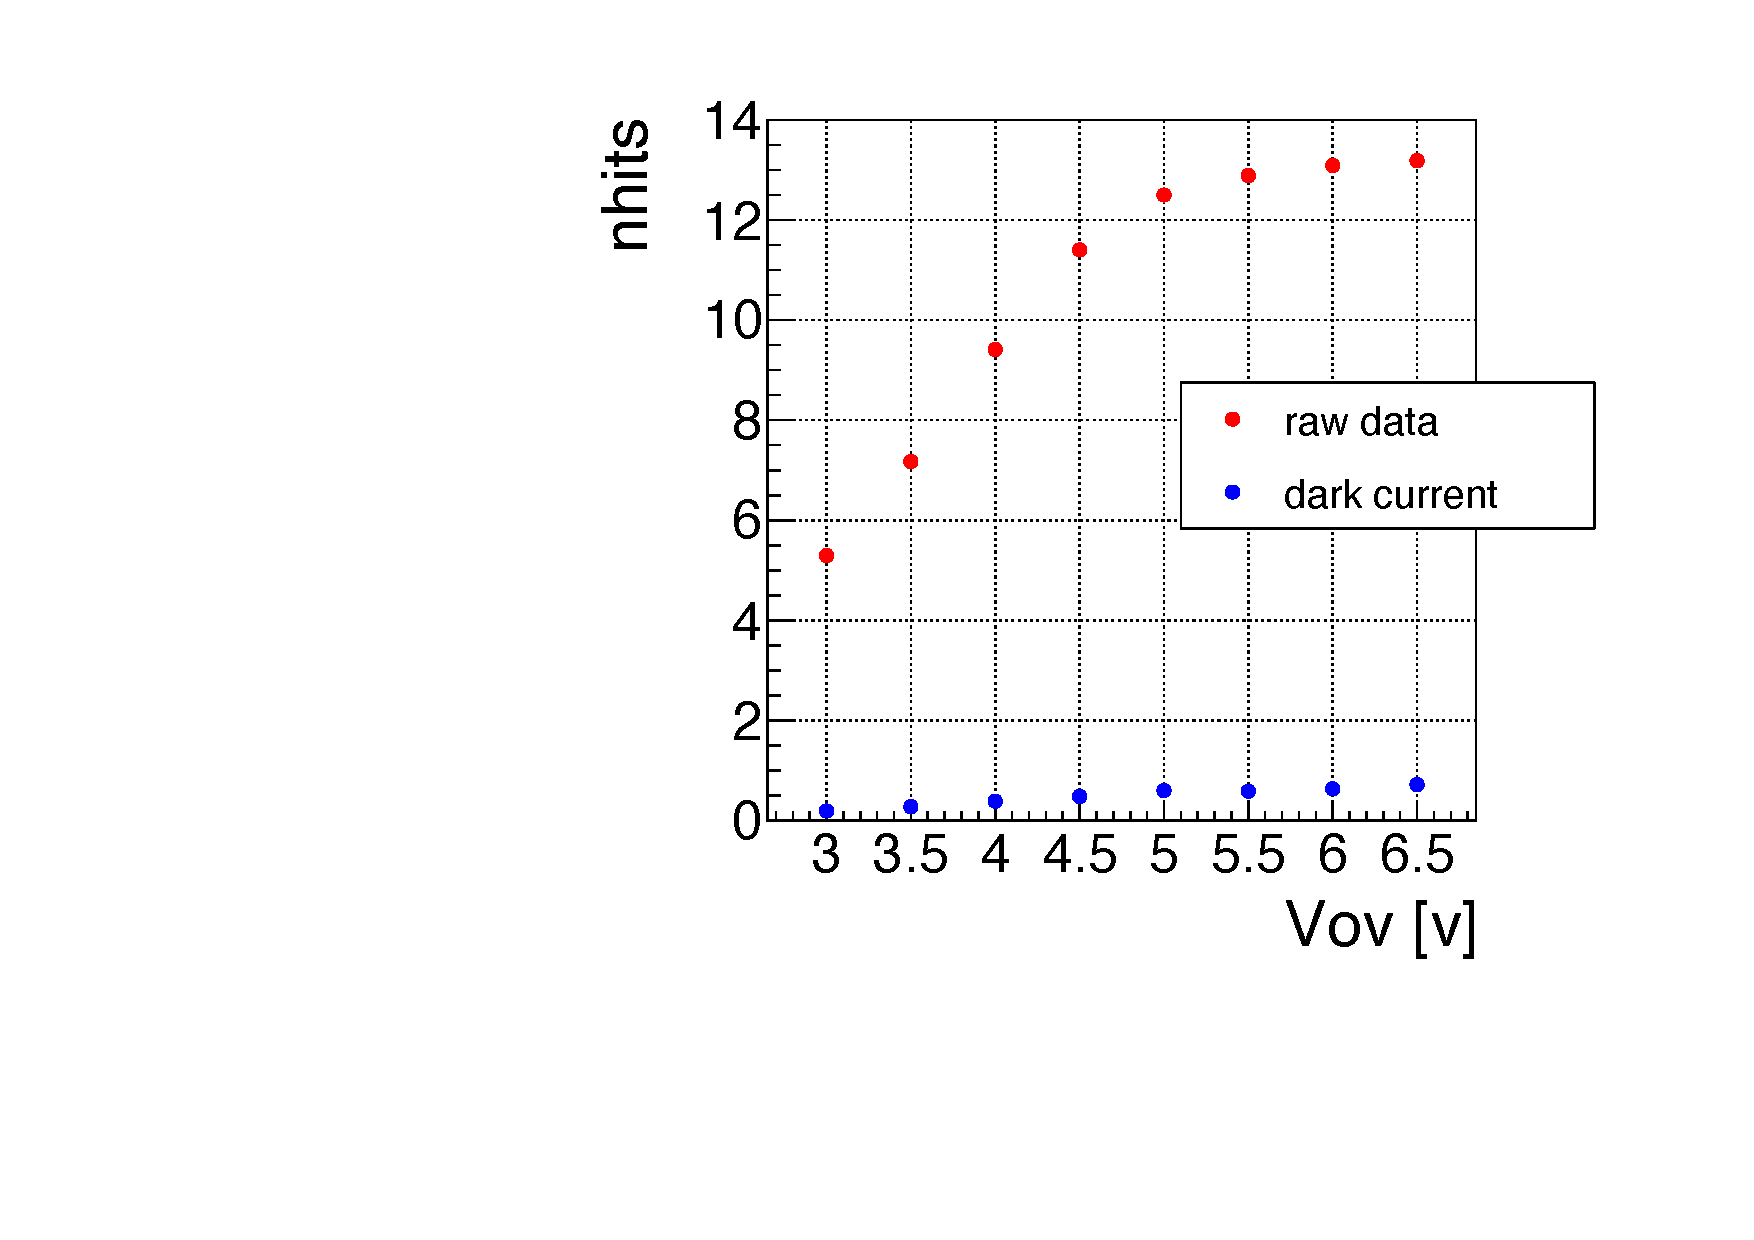
\includegraphics[scale=0.36, clip]{image/hit_count.pdf}
          \caption{信号と暗電流のhit数} 
          \label{fig:hit_dark} 
        \end{minipage} &
        %---- 2番目の図 --------------------------
        \begin{minipage}[t]{0.45\hsize}
          \centering
          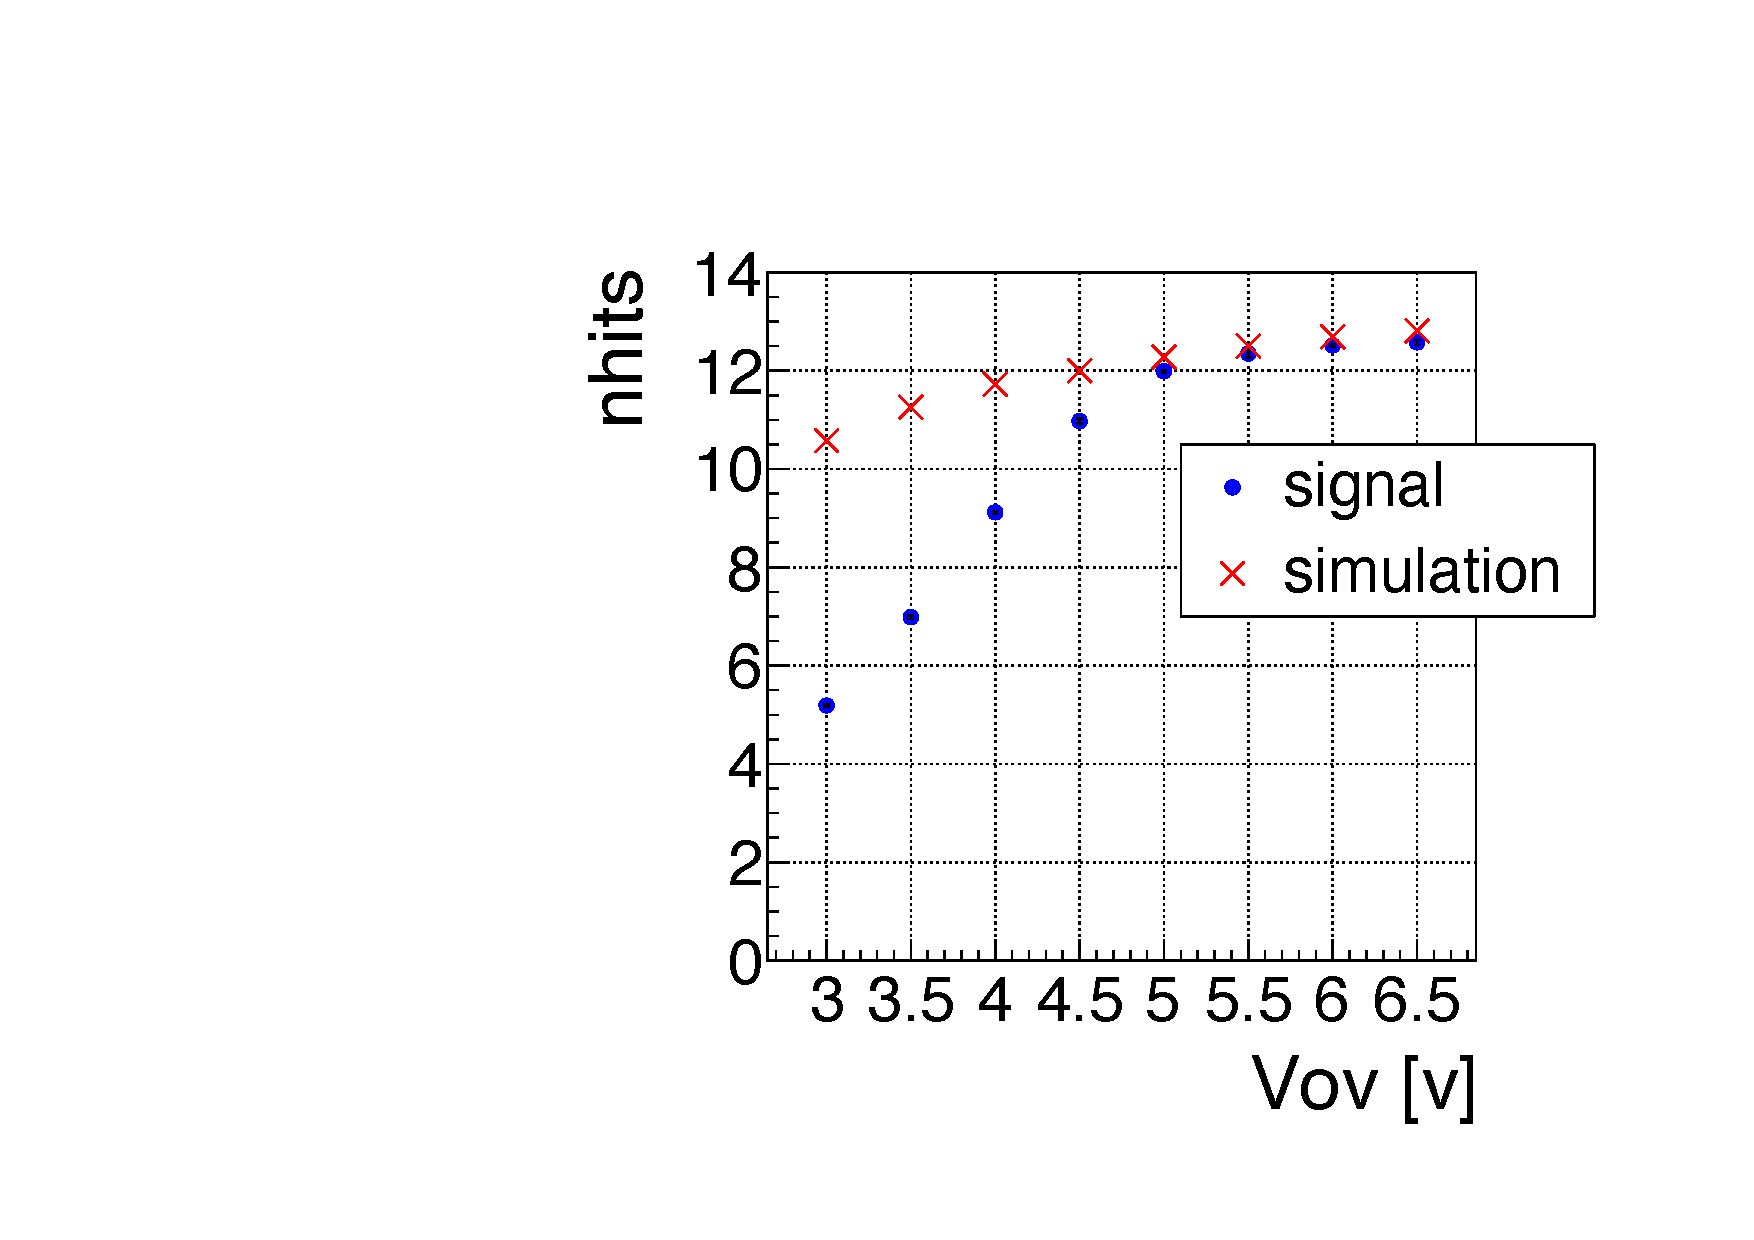
\includegraphics[scale=0.35, clip]{image/hit_simulation.pdf}
          \caption{信号とsimulationのhit数} 
          \label{fig:hit_simulation} 
        \end{minipage}
        %---- 図はここまで ----------------------
      \end{tabular}
    \end{figure}
    
    % \end{figure}

  \section{リング半径とチェレンコフ角}
    各電圧でのチェレンコフ角とリング半径は図$\ref{fig:all_theta}$と$\ref{fig:all_radius}$のようになった。
    \begin{figure}[hbtp]
      \begin{tabular}{cc}
        %---- 最初の図 ---------------------------
        \begin{minipage}[t]{0.45\hsize}
          \centering
          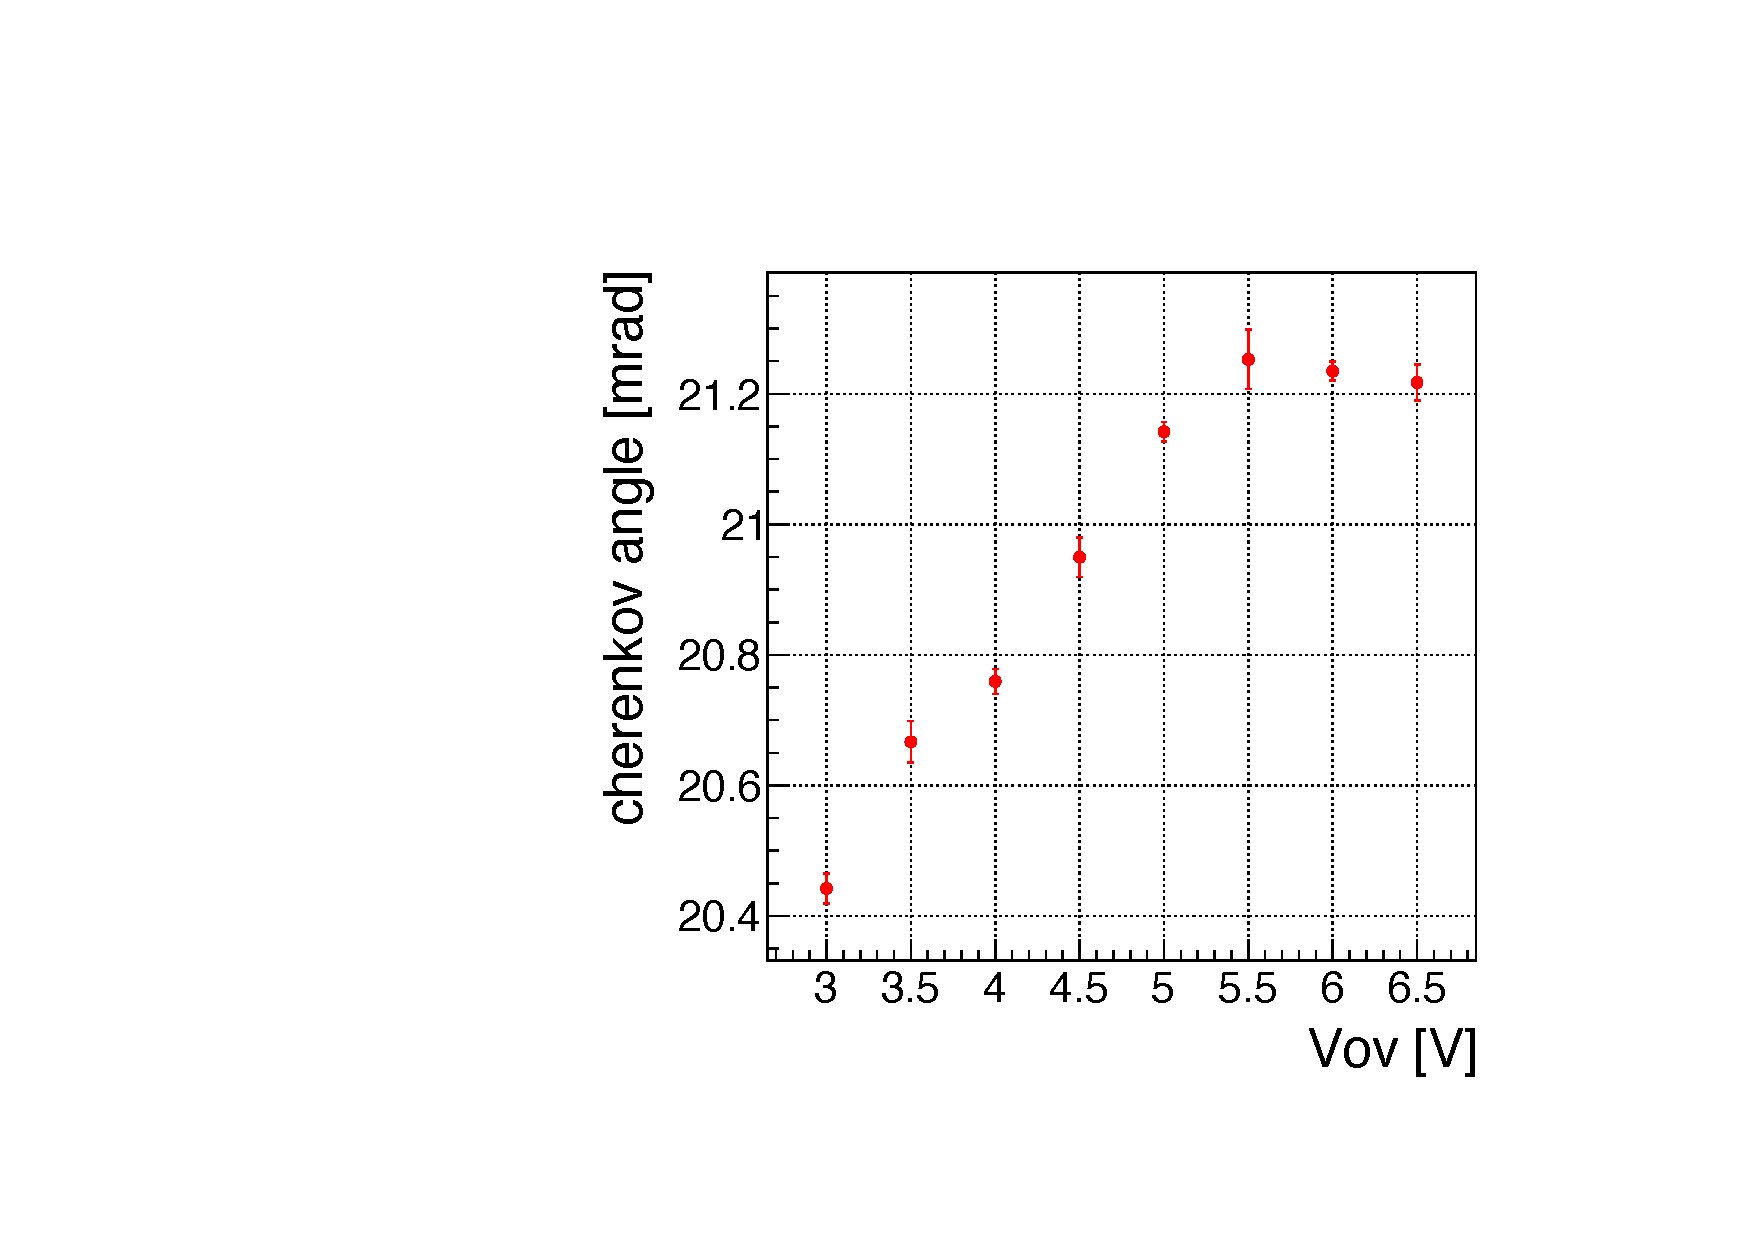
\includegraphics[scale=0.4, clip]{image/theta_allV.pdf}
          \caption{各電圧でのチェレンコフ角} 
          \label{fig:all_theta} 
        \end{minipage} &
        %---- 2番目の図 --------------------------
        \begin{minipage}[t]{0.45\hsize}
          \centering
          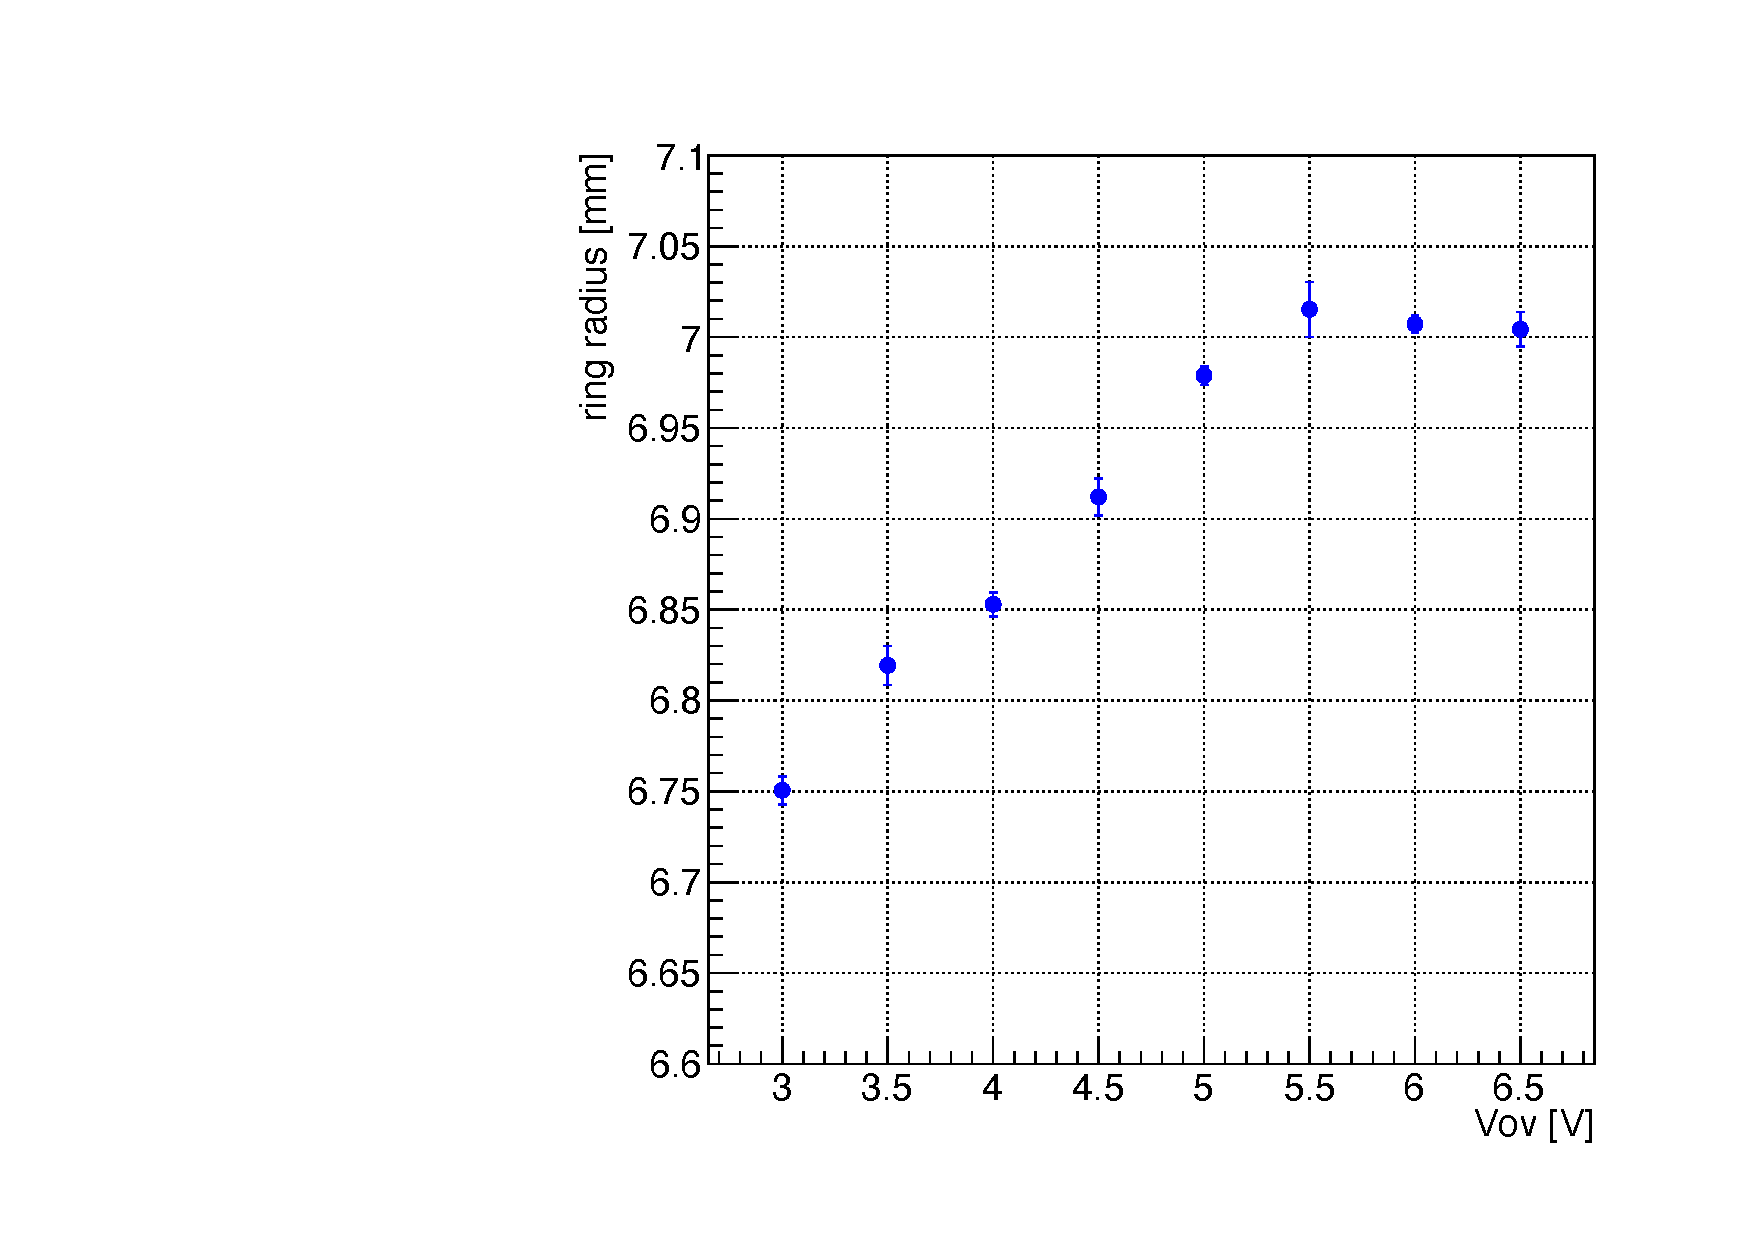
\includegraphics[scale=0.3, clip]{image/all_radius.pdf}
          \caption{各電圧でのリング半径} 
          \label{fig:all_radius} 
        \end{minipage}
        %---- 図はここまで ----------------------
      \end{tabular}
    \end{figure}


    \subsection{リング半径とチェレンコフ角の絶対値のズレ}
    まず、得られたチェレンコフ角・リング半径の絶対値について考える。
    ただし、チェレンコフ角とリング半径は式(\ref{theta_radius})より1対1対応なので、ここではリング半径について考える。
    MPPCが球面鏡の焦点面に配置されていた場合、MPPC上でのリング半径$r$は球面鏡の焦点距離$f=\SI{330}{mm}$、チェレンコフ角$\theta_{c}$から$r=f\tan{\theta_{c}}$とかける。
    今回は$\SI{0.95}{GeV/c}$の電子(陽電子)を用いたので、速度$\beta$は、相対論の式より
    \begin{eqnarray}
      p &=& \frac{mv}{\sqrt{1-{\beta}^2}} \nonumber \\
      pc &=& \frac{mc^2\cdot \beta}{\sqrt{1-{\beta}^2}} \nonumber 
    \end{eqnarray}
    よって、
    \begin{eqnarray}
      \beta &=& \sqrt{\frac{{pc}^2}{\left(mc^2\right)^2 + {pc}^2}} \nonumber \\
      &=& \sqrt{\frac{\left(0.95\times 10^9\right)^2}{\left(0.51\times 10^6\right)^2 + \left(0.95\times 10^9\right)^2}} = 0.999 \nonumber
    \end{eqnarray}
    となる。
    この時、チェレンコフ角$\theta$は空気の屈折率を$n=1.000273$とすると、式(\ref{cherenkov})より
    $r=\SI{7.7}{mm}$となる。この値は解析で得られた値より10\%程度大きいが、
    今回の実験ではMPPCの配置が球面鏡の焦点面から$\SI{42}{mm}$ズレていたので、それが原因ではないかと考えた。
    このズレによる影響を、簡単のために光軸が球面鏡に垂直となる場合で考えた。
    図\ref{fig:optical_system}のように、MPPCが焦点面からズレていた場合焦点面で収束されるはずの光が内側と外側に広がってしまい、
    上流側の光(青色の線)が多いほどリングの内側にくる光が多くなる。今回のセットアップのMPPCの位置のズレを考慮して計算を行うと表$\ref{tab:radius}$のようになった。
    この平均値(avg)が実験データの解析で得られる値と考えると、先ほどとは逆に解析値の方が5\%ほど大きくなっている。\\
    \begin{figure}[hbtp]
      \begin{center} 
        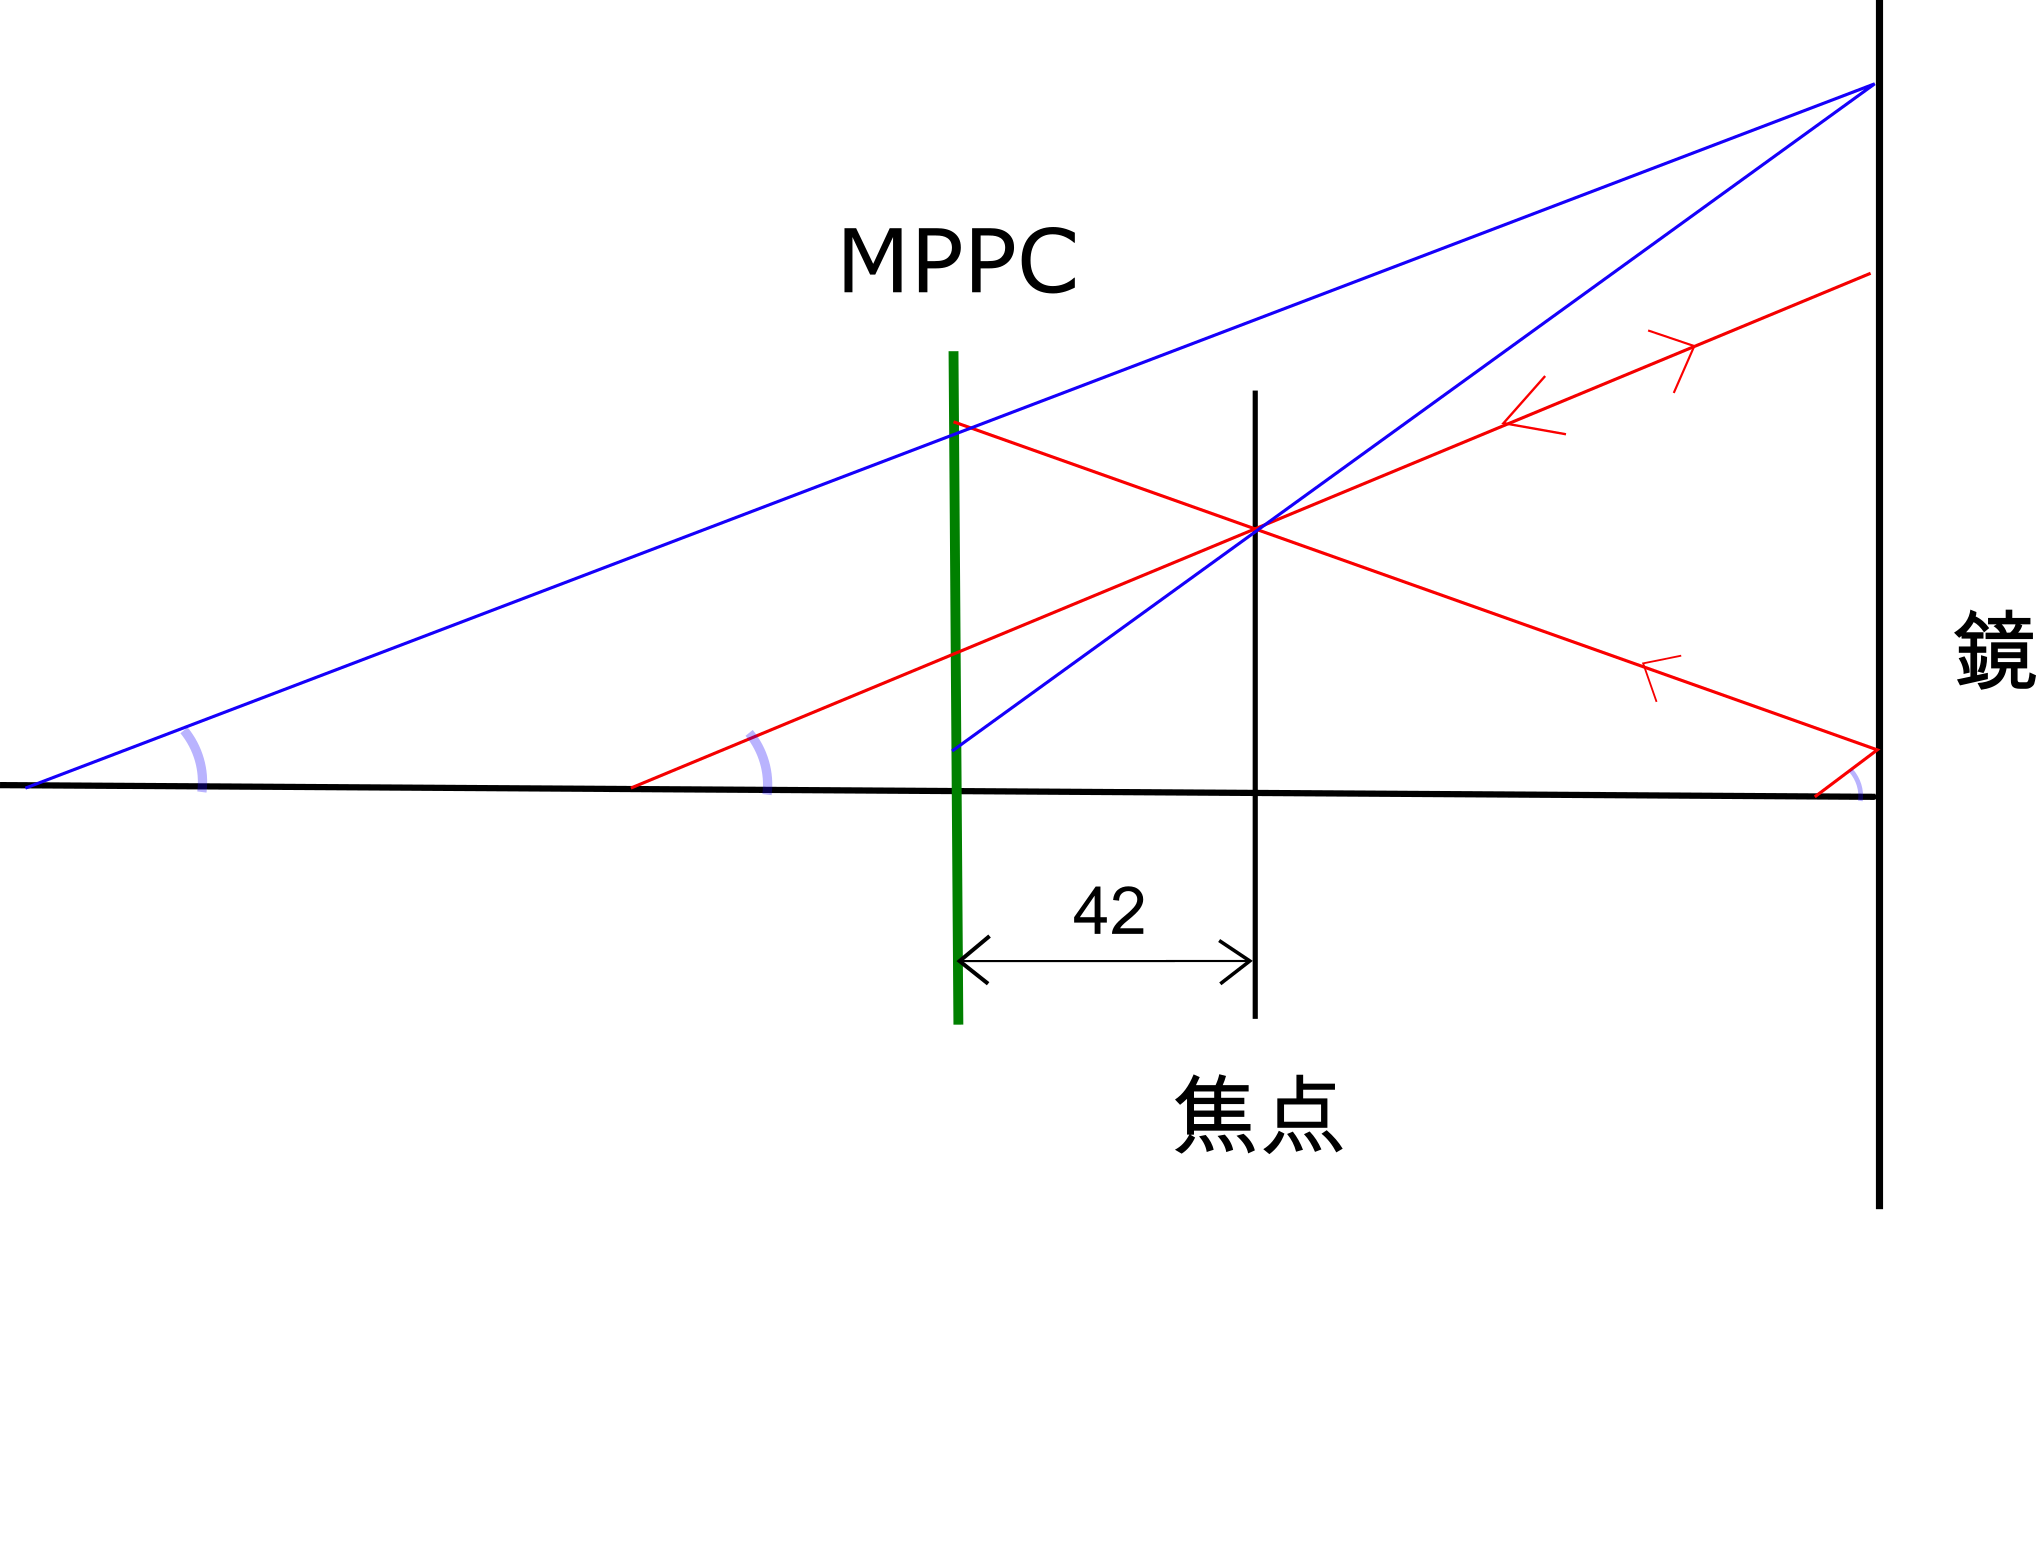
\includegraphics[scale=1, clip]{image/optical_system.png}
        \caption{光軸が球面鏡に垂直となる場合のイメージ図。} 
        \label{fig:optical_system} 
      \end{center}
    \end{figure}
    \begin{table}[hbtp]
      \begin{center}
        \label{tab:radius}
        \caption{リング半径の広がり。}
        \begin{tabular}{|c|c|c|}\hline
          min & avg & max\\ \hline
          \SI{4.54}{mm} & \SI{6.62}{mm} & \SI{8.69}{mm}\\ \hline
        \end{tabular}
      \end{center}
    \end{table}
    \begin{figure}[hbtp]
        \begin{center} 
          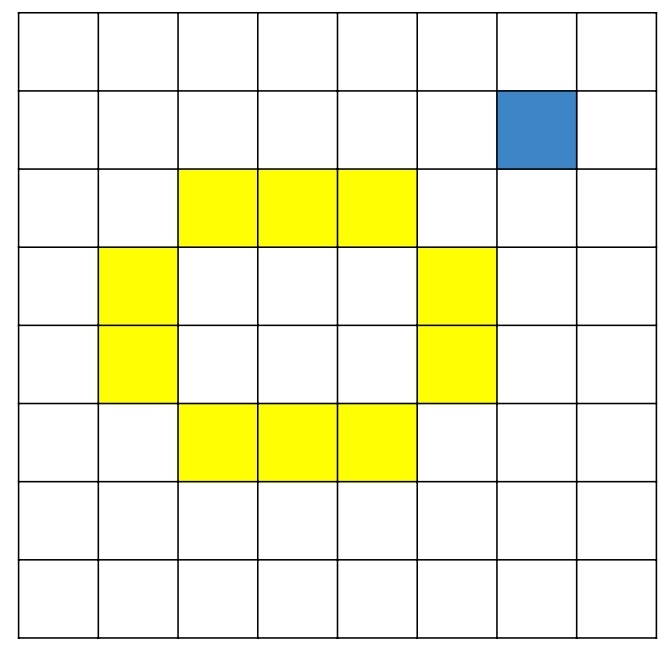
\includegraphics[scale=0.4, clip]{image/dark_current_image_page.jpg}
          \caption{黄:実際に光子が当たったセグメント、青:暗電流によるhitがあったセグメント。} 
          \label{fig:darkcurrent_image} 
        \end{center}
      \end{figure}
      逆に解析値の方が大きくなってしまう原因として考えられるのが、暗電流の効果である。
      例えば図$\ref{fig:darkcurrent_image}$のように、暗電流がリングの外側に出てしまった場合そのイベントのリング半径は実際よりも大きくなってしまう。
      リングの内側に暗電流が発生した場合はリング半径は小さくなるが、今回のリングとMPPCアレイのサイズ関係だと内側よりも外側の方が面積が大きいため、暗電流によってリング半径が大きく見積もられてしまう。
      図\ref{fig:darkcurrent_radius}は実際に暗電流のイベントのみの場合にリング半径を計算したものである。
      理論値よりも大きい値が得られることが分かる。
      \begin{figure}[hbtp]
        \begin{center} 
          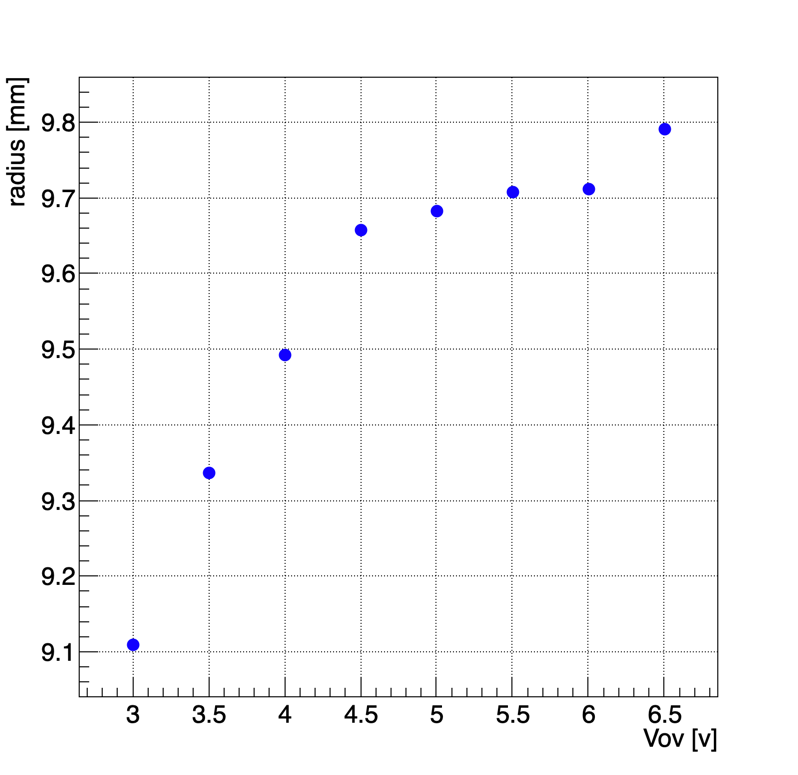
\includegraphics[scale=0.4, clip]{image/background_radius.png}
          \caption{暗電流のみでの各電圧のリング半径。}
          \label{fig:darkcurrent_radius} 
        \end{center}
      \end{figure}
    \subsection{リング半径・チェレンコフ角の電圧依存性}
    続いて、リング半径・チェレンコフ角の電圧依存生について考える。
    本来はMPPCの電圧を上げても、チェレンコフリングの半径やチェレンコフ角は一定のはずである。
    しかし、今回の実験ではMPPCの電圧を上げていくとリング半径・チェレンコフ角も増加していることが分かった。
    この電圧依存性の原因を考えるために、簡単なシミュレーションをおこなった。\\
    以下はそのシミュレーションの条件である。\\
    リング中心は$\left(x,y\right)=\left(3.3,3.9\right)$、リング半径は$4.54\sim\SI{8.69}{mm}$でランダムに生成した。
    1イベントごとの発生光子数は式(\ref{hit_count1})の計算より68個、MPPCの検出確率は浜松ホトニクスのホームページに記載の各電圧での値を用い、
    鏡の反射効率は全波長で$0.9$とした。
    また、1セグメントに複数の光子が同時に入る効果やセグメント間の隙間も考慮した。\\
    以上の条件で、実際の解析と同様の手順でリング半径を求めた。
    \begin{figure}[hbtp]
      \begin{center} 
        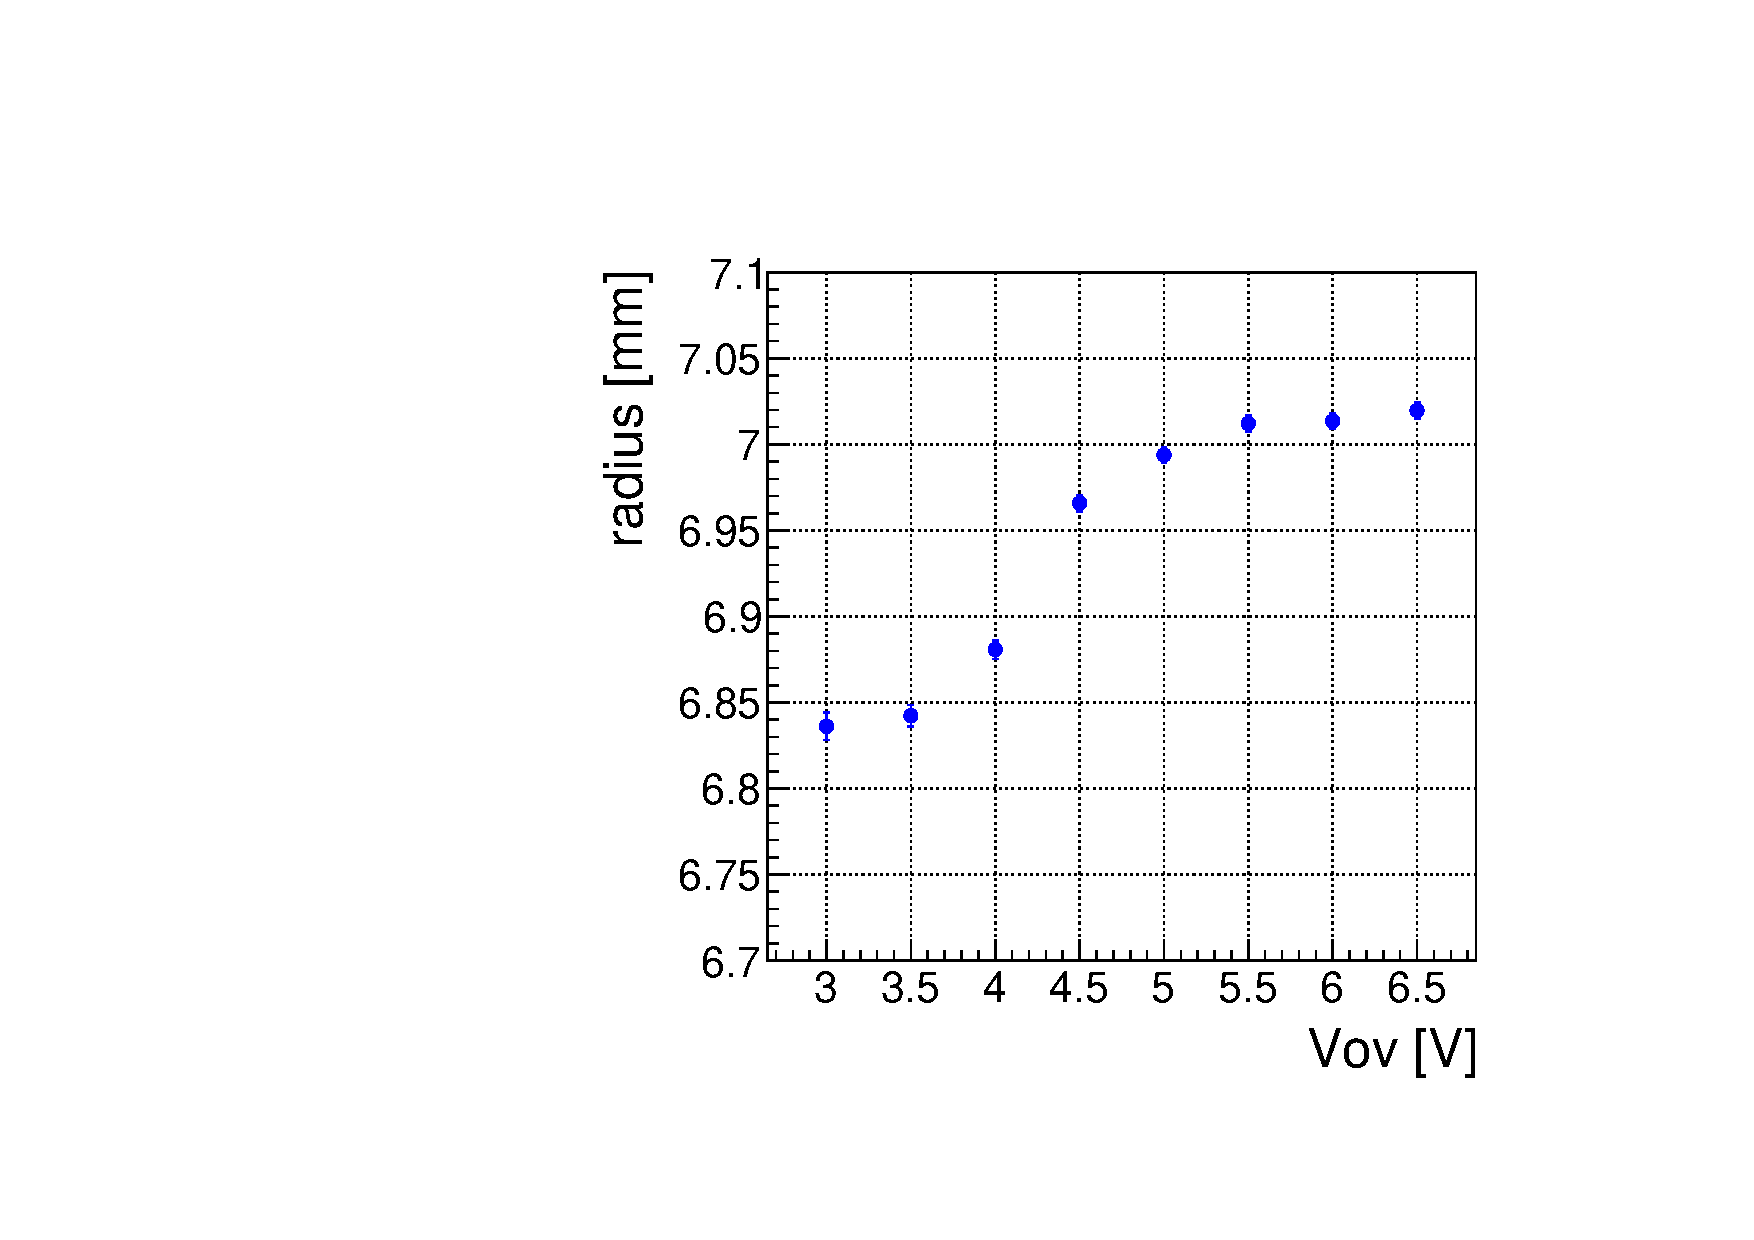
\includegraphics[scale=0.4, clip]{image/radius_simulation.pdf}
        \caption{シミュレーションによるリング半径。} 
        \label{fig:radius_simulation} 
      \end{center}
    \end{figure}
    図$\ref{fig:radius_simulation}$を見ると、シミュレーションでもリング半径に電圧依存性が見られることがわかる。
    これは暗電流の効果が原因と考えられる。
    図\ref{fig:darkcurrent_radius}から分かるように暗電流にはリング半径を大きくする効果があり、電圧を上げていくと暗電流が増加していくので、その効果が大きくなり、
    リング半径・チェレンコフ角に電圧依存性が生じてしまう。
  \section{角度分解能}
    各電圧での角度分解能をまとめると図$\ref{fig:resolution_all}$のようになった。
    分解能も$V_{ov}=\SI{5}{V}$あたりでサチュレーションしていることがわかる。
    \begin{figure}[htbp]
      \begin{center} 
        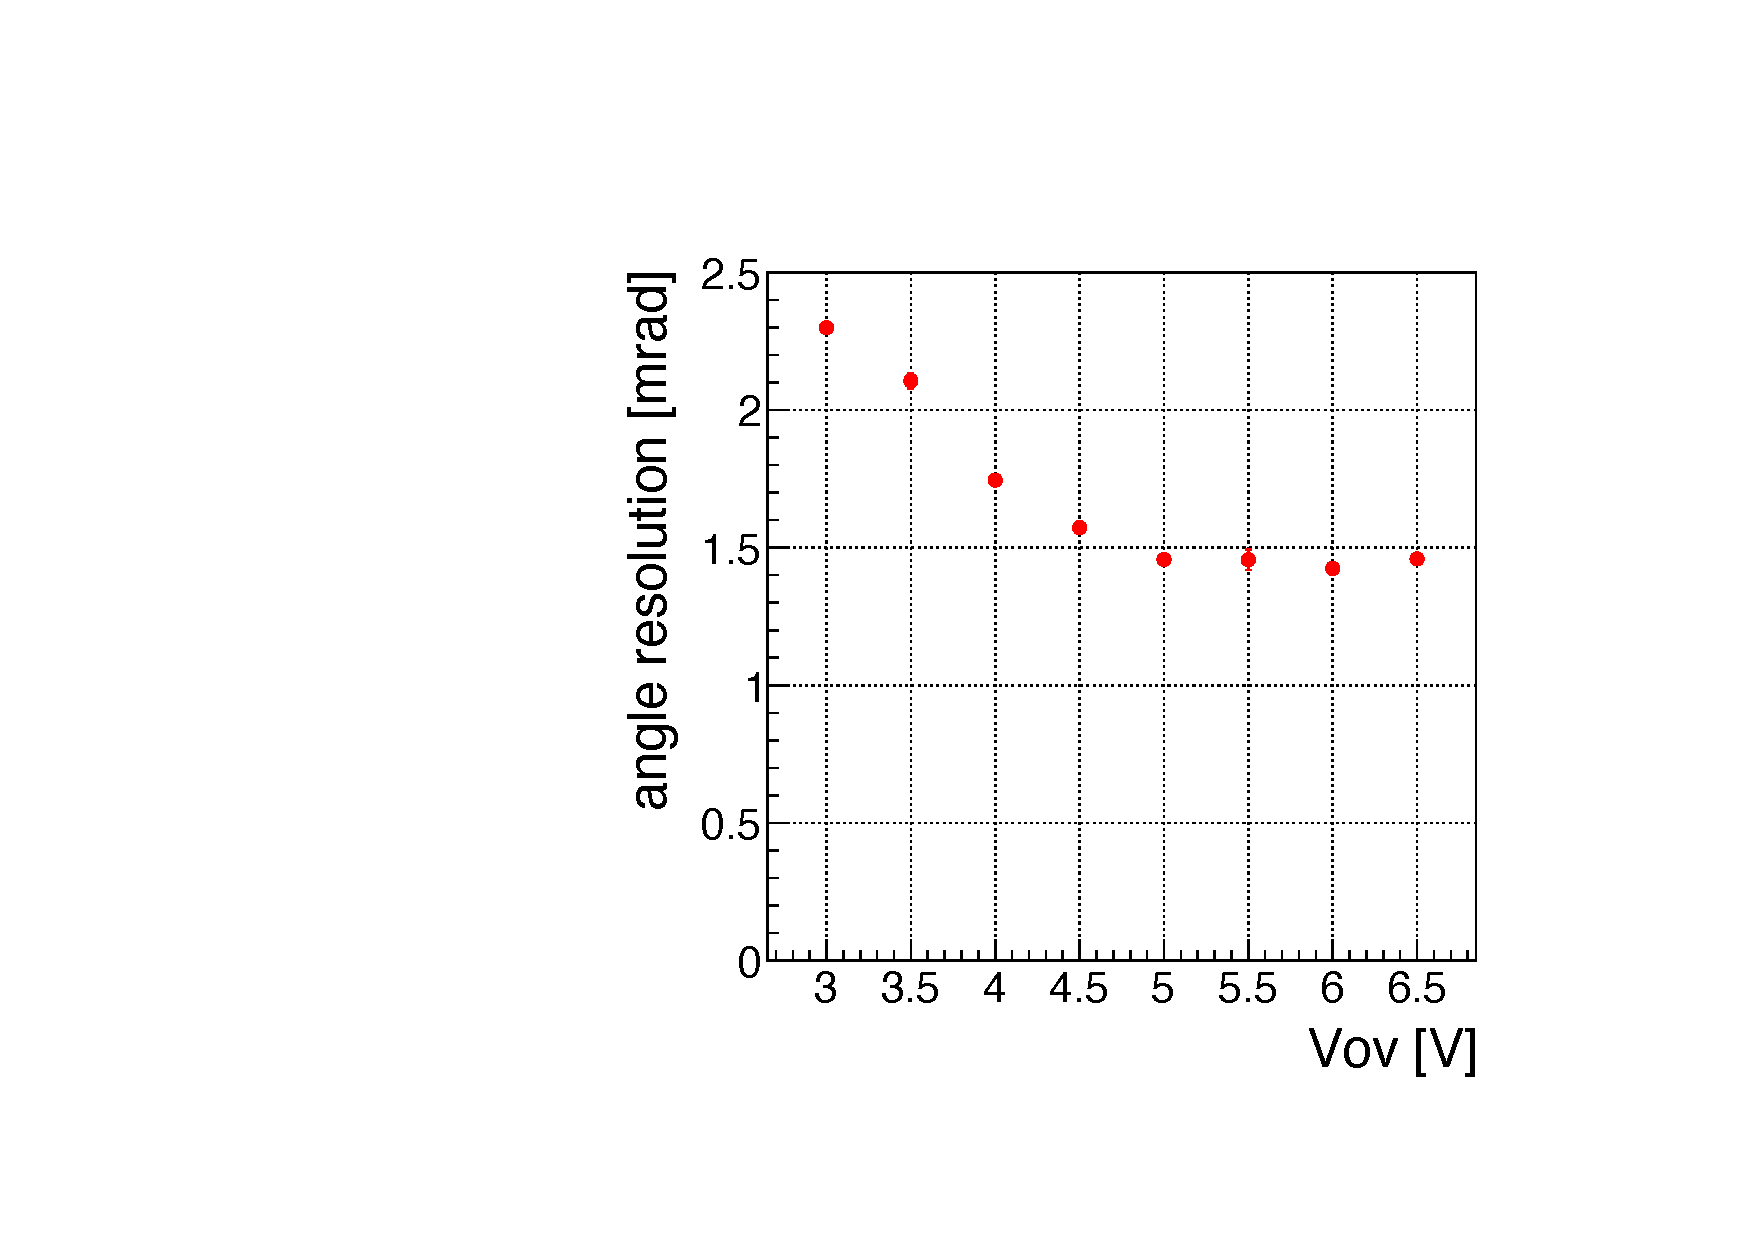
\includegraphics[scale=0.4, clip]{image/resolutin_allV.pdf}
        \caption{各電圧での角度分解能。} 
        \label{fig:resolution_all} 
      \end{center}
    \end{figure}

    \subsection{1 p.e.あたりの分解能}
    1 p.e.あたりの分解能を求めるために、イベントごとのhit数で場合分けをし分解能を求めた。
    さらに、1 p.e.あたりの分解能を$\Delta \theta_{1 p.e.}$として、$\frac{\Delta \theta_{1 p.e.}}{\sqrt{nhits}}$でフィッティングを行うと、
    図\ref{fig:per_hit}のようになった。
    フィッティングのパラメータの値より、$\Delta \theta_{1 p.e.} = 4.85 \pm 0.01 \: \si{mrad}$と求められた。
    \begin{figure}[htbp]
      \begin{center} 
        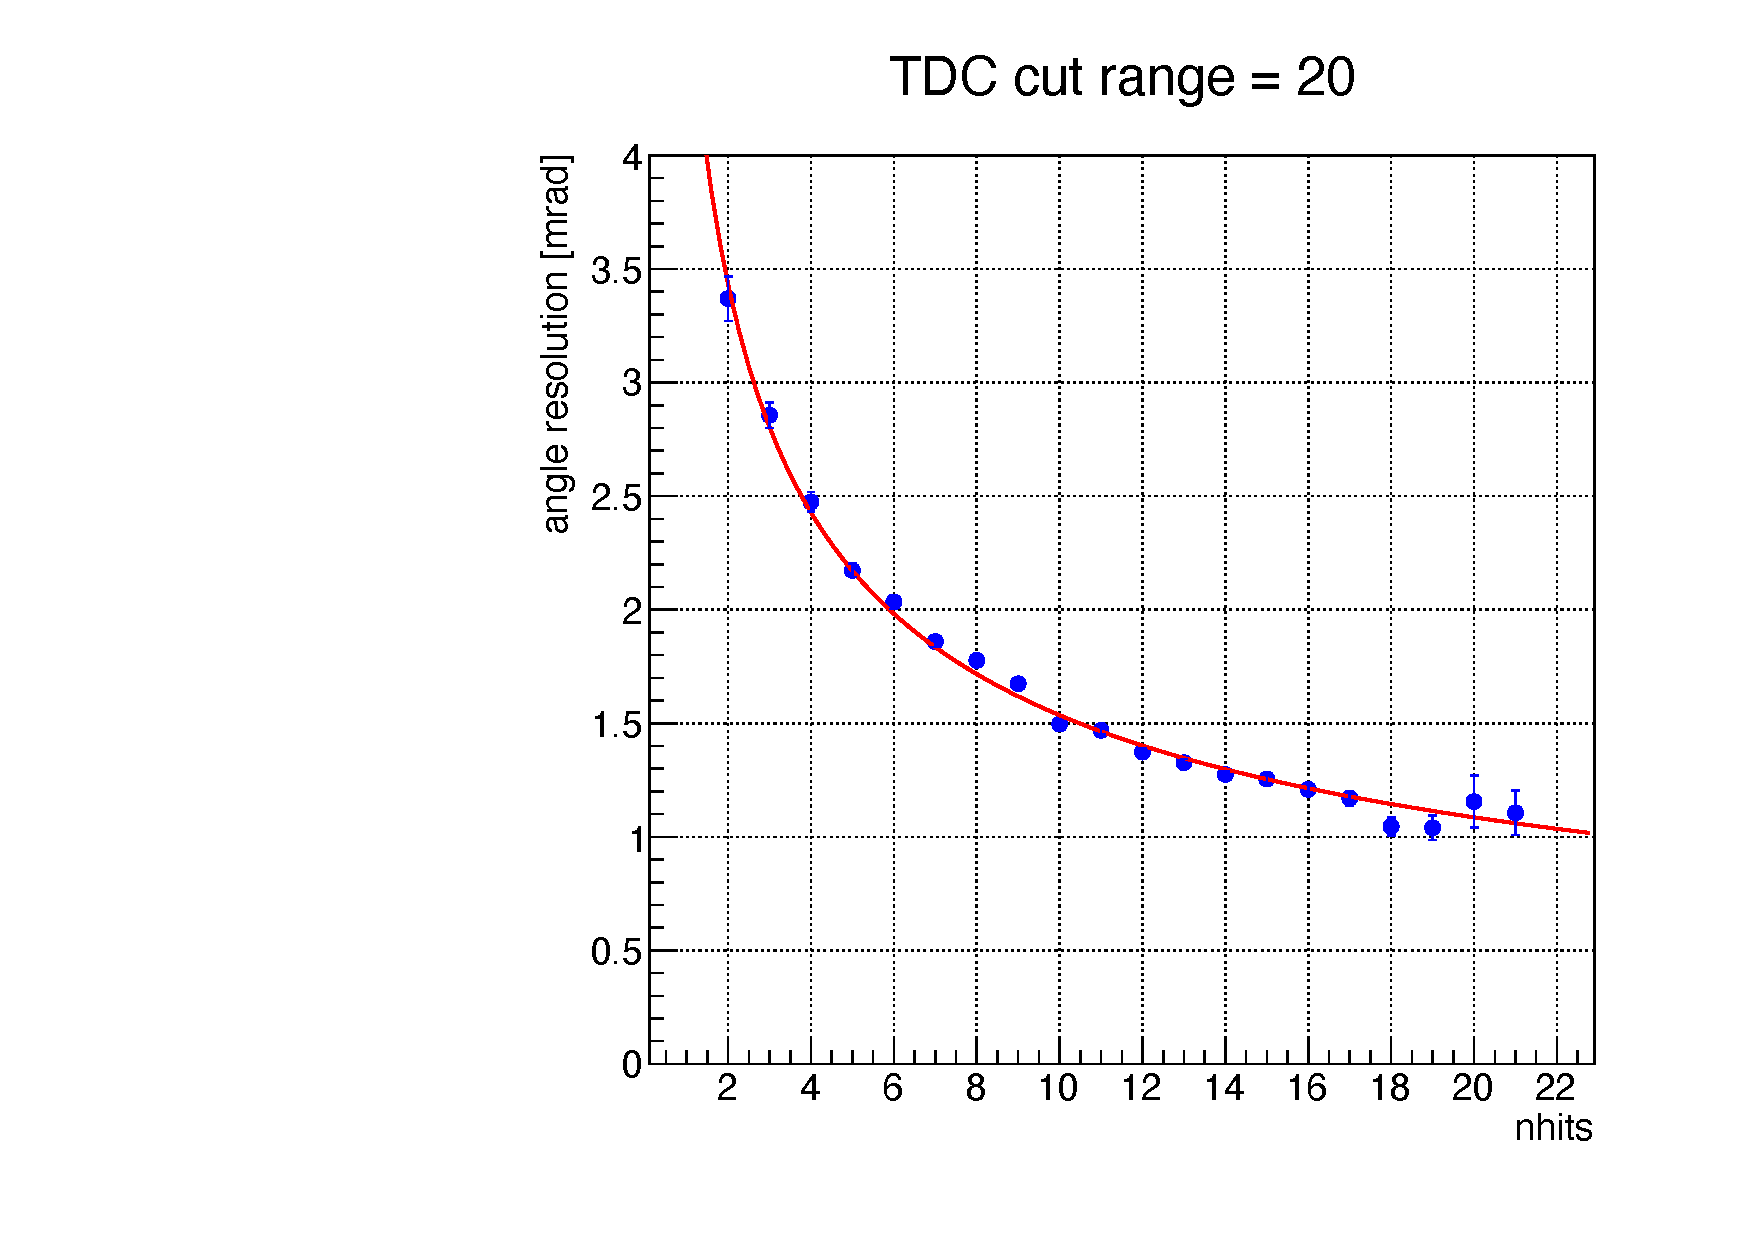
\includegraphics[scale=0.3, clip]{image/per_hit.pdf}
        \caption{hit数ごとの角度分解能。横軸はイベントごとのhit数、縦軸はチェレンコフリングの角度分解能。} 
        \label{fig:per_hit} 
      \end{center}
    \end{figure}
    
    
    
    \subsection{角度分解能の内訳}
    
    \subsection{収差などによる角度分解能}
    
    \subsection{暗電流の角度分解能への寄与}
    暗電流の角度分解能への影響を調べるために、暗電流がある場合と、暗電流なしの極限(TDCのcut幅を0にした極限)での角度分解能と1 p.e.あたりの分解能をそれぞれ調べた。
    まず、TDCのcut幅を100 chまで20 chずつ広げていき暗電流の割合を増加させた時の分解能を調べることで、暗電流なしの極限での角度分解能を外挿により求めた。
    図\ref{fig:reso_tdc}で、cut幅0つまり暗電流なしの極限を見ると$\sim\SI{1.38}{mrad}$の分解能が得られる。
    また、角度分解能と1 p.e.あたりの分解能の関係式$\frac{\Delta \theta_{1 p.e.}}{\sqrt{nhits}}=\Delta \theta$より、cut幅20の場合から$\sqrt{nhits}$が求まる。
    \begin{eqnarray}
      \frac{\SI{4.85}{mrad}}{\sqrt{nhits}}&=&\SI{1.45}{mrad} \nonumber \\
      \sqrt{nhits} &=& 3.34 \nonumber 
    \end{eqnarray}
    よって、cut幅0での1 p.e.あたりの分解能$\Delta \theta_{1 p.e.}$は$\frac{\Delta \theta_{1 p.e.}}{\sqrt{nhits}}=\SI{1.38}{mrad}$より
    $\Delta\theta_{1 p.e.}=\SI{4.62}{mrad}$となる。
    \begin{figure}[h]
      \begin{center} 
        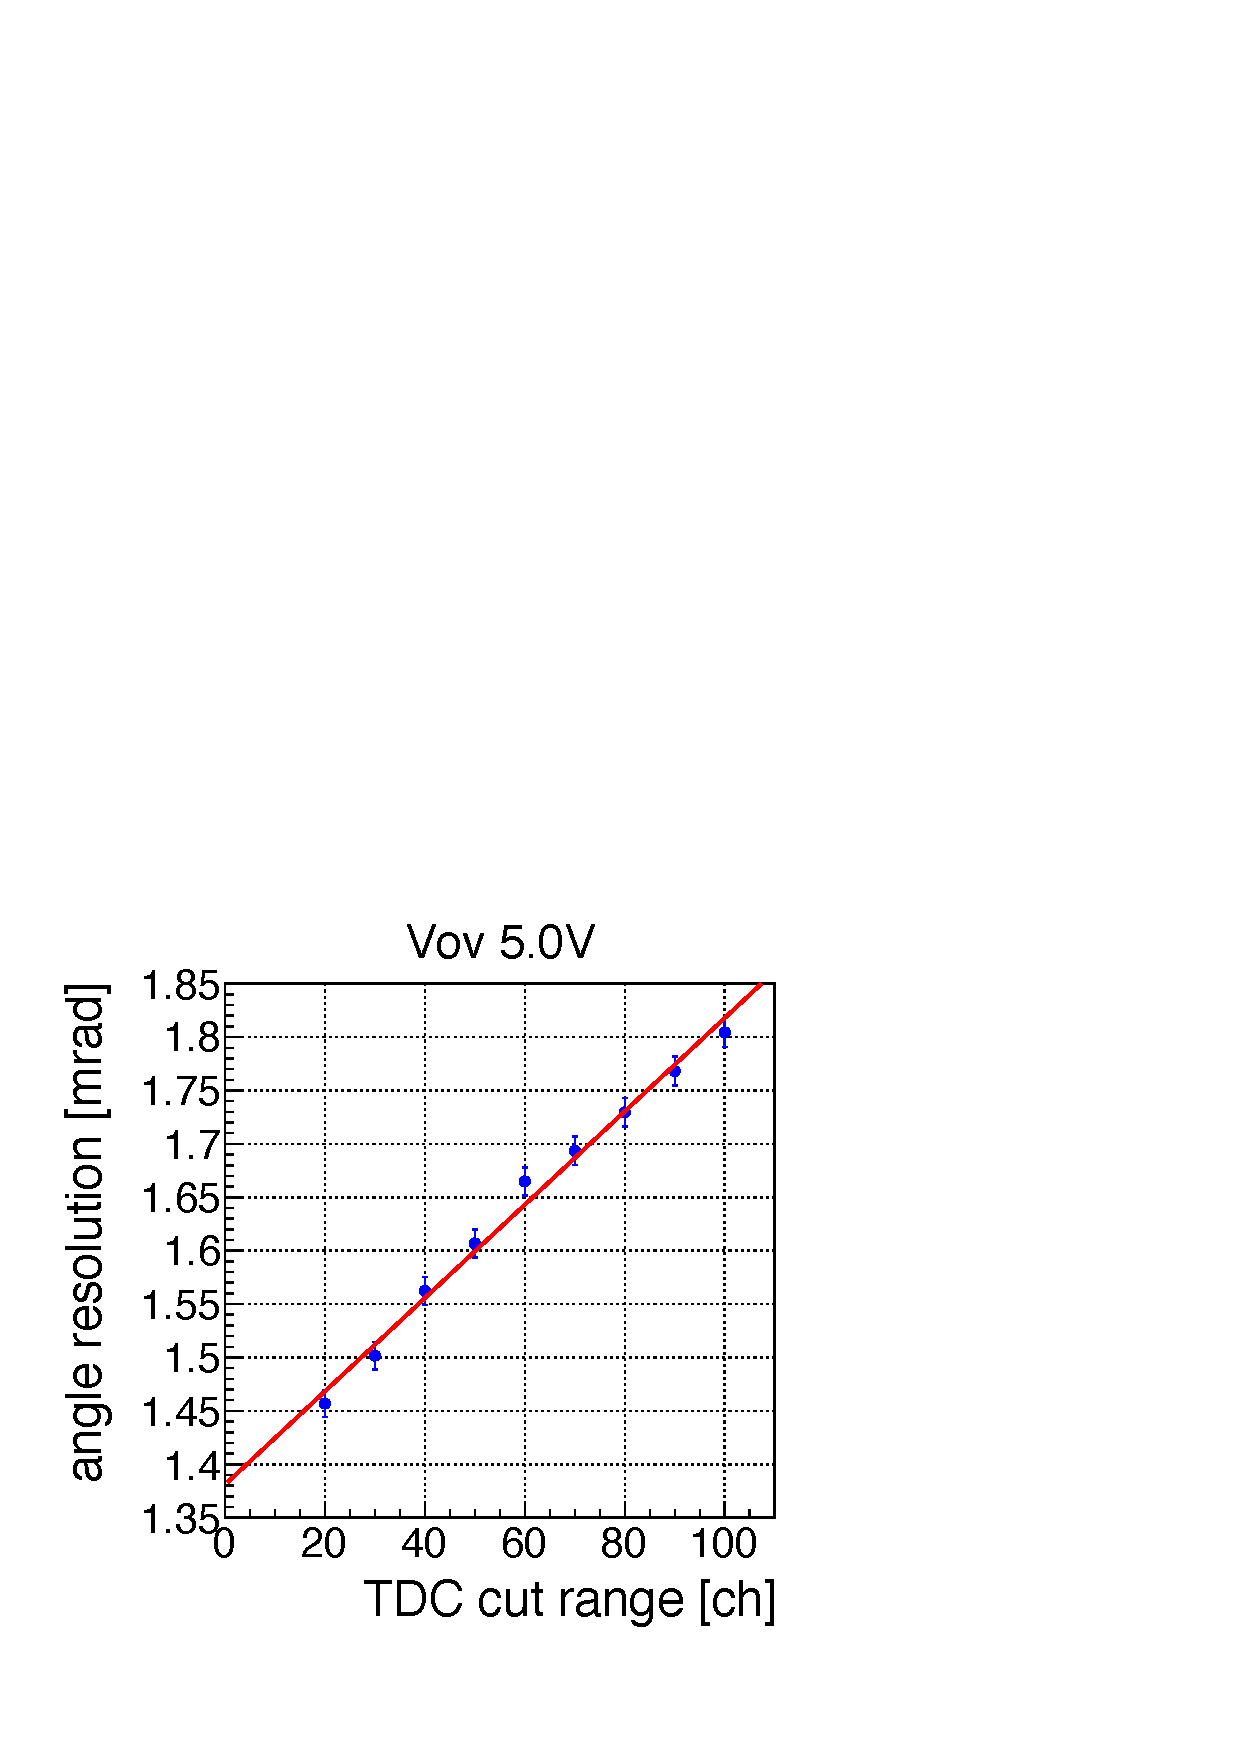
\includegraphics[scale=0.4, clip]{image/reso_tdc.pdf}
        \caption{TDCのcut幅を広げていった時の分解能の変化。} 
        \label{fig:reso_tdc} 
      \end{center}
    \end{figure}

\chapter{まとめ}
    J-PARC$\;$E50実験で研究するチャームバリオン分光では広い運動量領域$\left(2\sim16\;\si{GeV/c}\right)$での粒子識別が必要となるので、
    広い運動量領域に対応できるリングイメージング・チェレンコフ(RICH)検出器を用いる。
    今回は、球面鏡を使用したテスト機によってMPPCの暗電流の影響や電圧依存性、収差の角度分解能への影響を研究した。
    まず暗電流の寄与は、TDC cutで十分抑制可能ではあるが、1 p.e.あたりの分解能への影響が$\sim1.47\si{mrad}$程度あり、
    セグメントサイズが13\%程度大きく見えてしまう効果となることがわかったので、実機では暗電流の効果も含めてセグメントサイズを決定する必要がある。
    MPPCの電圧依存性については、hit数や分解能のサチュレーションしている値から$V_{ov}=\SI{5}{V}$あたりでの使用が良いとわかった。
    また、暗電流の効果によって、リング半径やチェレンコフ角に電圧依存性が生じるため、実機を使用する際はデータによるチェレンコフ角の較正が必要となることが分かった。

\chapter{参考文献}

\chapter{謝辞}
\end{document} 